%%
%% paper04 — 独立小论文稿(中文)
%% 模板: ACM acmart manuscript。正文已与旧 NOSR/HMACSP 叙事脱钩,仅保留版式骨架。
%% 编译: XeLaTeX(必须;见下方 ctex 说明)。
%%
\documentclass[manuscript,screen,review]{acmart}

%% ===================== 中文支持 =====================
%% scheme=plain: 只接管中文字体与断行,不改写 acmart 的章节名。
%% fontset=windows: 本机宋体/黑体; Overleaf/Linux 可改为 fontset=fandol。
\usepackage[UTF8,scheme=plain,fontset=windows]{ctex}

\usepackage{algorithm}
\usepackage{algorithmicx}
\usepackage{algpseudocode}
\usepackage{pifont}
\usepackage{makecell}
\providecommand{\checkmark}{\ding{51}}
\newcommand{\cmark}{\ding{51}}
\newcommand{\xmark}{\ding{55}}
\newcommand{\omark}{\(\circ\)}
\usepackage{threeparttable}
\usepackage{tikz}
\usetikzlibrary{positioning,arrows.meta,calc,shapes,shadows}
\usepackage{xcolor}
\usepackage{amsmath}
\usepackage{bm}
\DeclareMathOperator*{\argmin}{arg\,min}
\DeclareMathOperator*{\argmax}{arg\,max}
\usepackage{multirow}
\usepackage{enumitem}
\usepackage{booktabs}
\usepackage{graphicx}
\setlength{\headheight}{20.48303pt}

%% 机制缩写:主语是闭包,不是「修复框架」
\providecommand{\STRC}{\textsc{STRC}}
\newcommand{\TBD}[1]{\textcolor{red}{\textbf{[待补:} #1\textbf{]}}}

%% =====================================================================
%% 主结果数字的单一来源。
%%
%% 全部由 STRC/tools/paper_numbers.py 从 STRC/experiments/expanded/*.csv 打印,
%% 数据由 `py -m tools.expand_batch` 生成(默认 5 算例 x 10 种子)。
%% 正文一律用宏,不写字面量;改数只改这里,并同步跑一遍上述两条命令核对。
%%
%% !! 2026-08-16 由 3x5=15 对扩到 5x10=50 对。旧稿所有 /15 读数一律作废。
%%
%% !! 2026-08-16(二次):E2b 由 24/50 变为 50/50。这不是换了算例,而是修掉了
%% !! 一处实现与定义的错配。释放集是一个**预约**集合,而 replay_reroute 原先
%% !! 按**工序**判定是否重路(两段中任一段进闭包就整道重规划)。于是当只有满载
%% !! 段进闭包时,同工序的空载段也被改写,而它的 task 并不在释放集里,遂被记为
%% !! 外侧漂移。26 个失败格上的 84 条漂移预约无一例外都是这种同工序空载段,
%% !! 其中 71 条(85%)在 t_now 之前就已执行完毕——改写它同时违反假设 A2。
%% !! 改为按段判定后漂移归零。据此 prop:outside 的前提 (iii) 才真正被满足,
%% !! 此前的 24/50 测的是实现缺陷,不是边集的物理覆盖度。
%% =====================================================================
\newcommand{\NInst}{5}
\newcommand{\NSeeds}{10}
\newcommand{\NPairs}{50}
%% E1/E3:两项都是满分,写成 \NPairs/\NPairs 以免手抄漏改
\newcommand{\PassMiss}{\NPairs/\NPairs}      % T_impact=0 且种子非空且原解不可行
\newcommand{\FeasRone}{0/\NPairs}            % R1 恢复可行的格数
\newcommand{\FeasRtwo}{\NPairs/\NPairs}      % R2 恢复可行的格数
\newcommand{\PassClosed}{\NPairs/\NPairs}    % E2a 结构闭合(泄漏为 0)
\newcommand{\PassInvar}{\NPairs/\NPairs}     % E2b 外侧字段逐条不变
%% 耗时(E3 批次,第 1 级改路、无扩域)
\newcommand{\MsRepairMed}{3.1}
\newcommand{\MsRepairMax}{15.0}
%% 稳定性(E5 批次):被改动预约占全表比例(两算例的区间,不取单点)
\newcommand{\ResFracRtwo}{57\%--60\%}
\newcommand{\ResFracRzero}{97\%--100\%}
%% E5 批次:全局重解臂改写的「已完成预约」占比(按 A2 应为 0)。取逐预算点的区间,
%% 不取种子均值——这里要说的是「无一点为零」,均值会把它糊掉。
%% 出处 STRC/experiments/e5_a2_audit.csv,由 `py -m tools.expand_batch --only-e5`
%% 生成(与 expanded/e5_cross_curve.csv 同协议同代码路径,只是多记四列越界计数;
%% 未覆盖官方文件是因为 R0+ 受挂钟预算约束、代数随机,重跑会改动 tab:e5 的读数)。
%% 同一文件里 R2 的越界计数在全部 18 点上为 0。
\newcommand{\RzeroPastLo}{80\%}
\newcommand{\RzeroPastHi}{100\%}
%% 规模扫描的加速比区间(跨两算例的逐格极值)
\newcommand{\SpeedLo}{87}
\newcommand{\SpeedHi}{3051}
%% E6:A 类上闭包严格大于任务图释放集的格数(其余格两者相等,不是包含失败)
\newcommand{\StrictlyLarger}{81/100}
%% E6:闭包占 t_now 之后活预约的比例(走廊阻断)。这个数偏大,
%% 是「不作最小性主张」那条注记的实测依据,不要美化。
\newcommand{\ClosureAliveFrac}{90\%}
%% =====================================================================
%% 外部来源布局批次(STRC/experiments/pub_layouts/)。**独立账本**,不并入上面的
%% \NPairs 对——把它混进主批次会让全部 /\NPairs 读数改口径。两批算例逐参数同口径,
%% 只差布局来源。数出处:py -m tools.pub_batch 后 py -m tools.paper_numbers。
%% 边权是本文补齐的等权值,故这批数**不可**与 Lyu 或 van Os 的参照值比较。
%% =====================================================================
\newcommand{\NPubInst}{5}
\newcommand{\NPubPairs}{50}
\newcommand{\PubPassMiss}{\NPubPairs/\NPubPairs}
\newcommand{\PubFeasRone}{0/\NPubPairs}
\newcommand{\PubFeasRtwo}{\NPubPairs/\NPubPairs}
\newcommand{\PubPassClosed}{\NPubPairs/\NPubPairs}
\newcommand{\PubPassInvar}{\NPubPairs/\NPubPairs}
\newcommand{\PubEoneFracLo}{0.438}
\newcommand{\PubEoneFracHi}{0.547}
%% E4 同参数对照。**这里的口径要格外小心,曾写错过一次。**
%% \NPubInst 个外部算例只落在 \NPubNets 张不同路网上(4x4 去一条边:LyuL2/L3;
%% 5x5 去两条边:LyuL4/L5/L6),差别在机器台数与落位。于是:
%%   \PubCloSpread 这个极差的两个端点(\PubCloHi=LyuL2 4 机、\PubCloLo=LyuL3 5 机)
%%   **共享同一张路网**,所以它测的是机器落位,**不是**路网几何。
%%   不要再写成"闭包占比随布局显著变化"——数据不支持这句。
%% 正确的用法是:同一路网上换落位即得 \PubCloSpread,而 LU 最小割与漏斗占比全程恒定
%% (两张路网都把装卸站放在网格角点,四邻接下角点恰两条出边),故静态割被干净否证。
%% 注意别把这句写成"公开布局一律放在角点":工具集另附的 Liu 那族放在网格边中点(出度 3),
%% 只是因允许对角移动而未收入。准确的说法是该指标只取到极少数由摆位决定的离散值。
\newcommand{\NPubNets}{2}
\newcommand{\PubCloLo}{0.305}
\newcommand{\PubCloHi}{0.512}
\newcommand{\PubCloSpread}{0.207}
\newcommand{\PubCloSpreadBig}{0.075}
\newcommand{\SelfCloLo}{0.446}
\newcommand{\SelfCloHi}{0.497}
\newcommand{\SelfCloSpread}{0.051}
\newcommand{\PubEfiveNoCross}{17/18}
%% =====================================================================
%% 便宜对照臂(E7)与算例规模扫描(E8)。两批共用同一组臂定义:
%%   RS  全局右移。不改路径/指派/序,把未完成的一切统一后推到阻断窗之后。
%%       冻结判据与 R2 相同(t_end <= t_now 不可动),故按 A2 可采纳。
%%   RD  原染色体重解码。保持机器指派与扫描序,在装了阻断的路由层上从头解一遍。
%%       **不受 A2 约束**,读它的 Cmax 必须连着 \RedecodeBad 一起读。
%%   RA  不划边界:释放 t_now 之后的全部预约,再走与 R2 完全相同的改路重放。
%%       它与 R2 共用引擎、共用冻结判据,唯一差别是释放集取了平凡上界,
%%       故 R2--RA 之差可全部归因于闭包这个对象本身。
%% 出处:STRC/experiments/cheap_baselines.csv (py -m tools.cheap_baselines)
%%      STRC/experiments/scale_curve.csv     (py -m tools.scale_curve)
%% 协议与 E1--E3 一致(繁忙走廊单窗阻断、t_now=0.35 Cmax、R2 不开扩域),
%% 故 tab:cheap 可与 tab:e3 并读;但**不可**与 tab:e5 并读——那批只有两个算例。
%% =====================================================================
\newcommand{\MsShift}{1.75}          % RS 耗时中位/ms(\NPairs 对)
\newcommand{\MsRedecode}{7.51}       % RD 耗时中位/ms(同上)
\newcommand{\MsAllFuture}{3.30}      % RA 耗时中位/ms(同上)
\newcommand{\MsCheapRtwo}{3.16}      % 同批 R2 的耗时中位,供四臂同口径比较
\newcommand{\ShiftBad}{0/\NPairs}    % RS 改写已完成预约的格数
\newcommand{\RedecodeBad}{31/\NPairs}
\newcommand{\WinVsShift}{27/16/7}    % R2 对 RS 的 Cmax 赢/平/输
\newcommand{\WinVsRedecode}{2/23/25}
\newcommand{\WinVsAllFuture}{4/46/0}
\newcommand{\ResFracCheapRtwo}{0.535}
\newcommand{\ResFracShift}{0.627}
\newcommand{\ResFracRedecode}{0.586}
\newcommand{\ResFracAllFuture}{0.604}
%% R2 对 RA 的逐格稳定性对比(改动比例;两臂都可行的 \NPairs 格全部纳入)。
\newcommand{\RAStabWTL}{32/17/1}     % R2 更稳/持平/更差
\newcommand{\RAStabP}{5.9\times10^{-7}}  % Wilcoxon 符号秩,双侧
\newcommand{\RAStabMean}{0.069}      % 改动比例平均降幅
\newcommand{\RAStabMed}{0.031}       % 同,中位降幅
\newcommand{\RACmaxRatio}{0.999}     % Cmax 比 R2/RA 均值
\newcommand{\RACmaxLo}{0.970}        % 同,最小值(R2 最占优的那格)
\newcommand{\ClosureShareLo}{0.77}   % 闭包/全部未来预约:最小值
\newcommand{\ClosureShareMean}{0.90} % 同,均值(与 \ClosureAliveFrac 同源)
%% 算例规模梯子:工件 2k、机器 k、车 k,k=4..10;拥堵档、H、F、Tt/Tp 与两处割集同口径,
%% 只有规模变(生成器 clbs/tools/gen_instances.py 的标定见其文档字符串)。
\newcommand{\ScaleKs}{7}
\newcommand{\ScalePairs}{70}
\newcommand{\ScaleJobsHi}{20}
\newcommand{\ScaleMachHi}{10}
\newcommand{\ScaleCloLo}{0.43}       % 闭包占全表比例:k=10
\newcommand{\ScaleCloHi}{0.54}       % 同,k=4
\newcommand{\ScaleMsHi}{11.8}        % R2 耗时中位:k=10
\newcommand{\ScaleRatioLo}{2.3}      % RD/R2 耗时比:k=4
\newcommand{\ScaleRatioHi}{5.5}      % 同,k=10
\newcommand{\ScaleFeasFirst}{69/\ScalePairs}   % 第 1 级改路即可行的格数
\newcommand{\ScaleFeasAll}{\ScalePairs/\ScalePairs}

\usepackage{amsthm}
\newtheorem{assumption}{假设}
\newtheorem{definition}{定义}
\newtheorem{problem}{问题}
\newtheorem{remark}{注}
\newtheorem{prop}{命题}
\newtheorem{lem}{引理}

\AtBeginDocument{%
  \providecommand\BibTeX{{%
    Bib\TeX}}}

\setcopyright{acmlicensed}
\copyrightyear{2026}
\acmYear{2026}
\acmDOI{XXXXXXX.XXXXXXX}

%%\acmSubmissionID{123-A56-BU3}

\begin{document}

%% =====================================================================
%% 标题:独立小论文用「任务图覆盖不到」钩子;大论文章题另用「闭包上的有界修复」
%% =====================================================================
\title[任务图覆盖不到的级联损坏]{任务图覆盖不到的级联损坏:无冲突柔性作业车间中的时空预约闭包}

\author{Qi Yu}
\email{230240012@seu.edu.cn}
\orcid{0009-0008-7843-6345}
\affiliation{%
	\department{School of Cyber Science and Engineering}
	\department{Key Laboratory of Computer Network and Information Integration}
	\institution{Southeast University}
	\city{Nanjing}
	\state{Jiangsu}
	\country{PR China}
}

\author{Wei Li}
\orcid{0009-0001-0949-329X}
\email{xchlw@seu.edu.cn}
\authornote{corresponding author}
\affiliation{%
	\department{School of Computer Science and Engineering}
	\department{Key Laboratory of Computer Network and Information Integration}
	\institution{Southeast University}
	\city{Nanjing}
	\state{Jiangsu}
	\country{PR China}
}

\renewcommand{\shortauthors}{Yu and Li}

%% =====================================================================
%% 摘要
%% 骨架:背景缺口 → 主张(边界在预约图) → 对象 STRC → 用法(有界修复) →
%%       与全局重解互补 → 实验钩子(不把创新挂在「又一个修复算法」上)
%% =====================================================================
\begin{abstract}
当柔性作业车间的运输被建模为常数时间矩阵时,车辆互不阻挡,延误只是布局属性;
一旦 AGV 在显式走廊网络上以时间窗预约通行,延误成为一车施加给另一车的量,
排程的可行性便同时写在任务依赖与预约表上。
\emph{在同时持有任务依赖图与显式走廊预约表的这一支调度文献中},
可继承的影响边界仍是受影响工序重调度(AOR)那一套——在\emph{任务依赖图}上界定:
由故障工序或故障智能体作种子,再按工序/指派邻域扩张。
这一做法覆盖一类扰动(机器故障、插单等),却系统性地漏掉另一类——
走廊阻断、路段降速等\emph{并不改动任何工序指派}的扰动。
对后者,任务图上直接受扰集合为空,框架会判「无需重调度」,而预约表上已有大片占用失效,
并沿「谁挡了谁」向外级联。本文把这一缺口表述为:\textbf{任务图覆盖不到的级联损坏}
——不是检测漏检,而是任务图这一表示本身不含预约级联通道。
该缺口只在两张图\emph{分立}的模型层级上存在:铁路调度的 alternative graph 把闭塞区段
即视为机器,两图合一;多智能体路径规划则没有任务图。

本文主张:在无冲突路由设定下,扰动的影响边界必须定义在\emph{时空预约图}上。
我们提出时空预约影响闭包(\STRC, Spatiotemporal Reservation Closure):
以与扰动时窗重叠的预约为种子,沿等待阻塞、同车接续、同工件接续与机器链等依赖取传递闭包,
得到可释放、可冻结的损坏范围。让行边与 alternative arc 同源,本文不主张它是新对象;
新的是它的\emph{用法}——不选择弧,而在既定排程之上取闭包,
使影响集从算法过程的副产品变为由图结构唯一确定的对象。
在闭包上做有界修复(改路,失败则扩大释放域)是把该对象用起来的手段;
「局部重规划 + 外侧冻结」与「失败扩域」两者在多智能体路径规划与局部重调度中均已是标准
做法,本文不以之为创新。

实验取 $5$ 算例 $\times$ $10$ 种子($50$ 个算例--种子对),在同一无冲突执行器与同挂钟协议下
对照任务图边界臂与热启动全局重解臂。走廊阻断上任务图影响域在 $50/50$ 上为空而闭包非空
且原排程不可行;同修复引擎下仅替换边界定义时,任务图边界 $0/50$ 恢复可行而闭包 $50/50$;
闭包的结构闭合性与闭包外侧字段的逐条不变均在 $50/50$ 上成立;
修复耗时中位 $3.1$\,ms,较热启动全局重解低两至三个数量级,
改动的预约为 $57\%$--$60\%$ 而后者为 $97\%$--$100\%$——
后一数字须带口径读:该对照臂并未受「已执行完毕的占用不可改写」约束,
它从 $t=0$ 重排,故其改动比例偏高、完工时间宜作参考下界。
对照不限于昂贵那一档:补入全局右移与原染色体重解码两档便宜的全局重算后,
唯一比有界修复更快的是\emph{不划边界}的右移,而它在完工时间与稳定性上都更差;
同一实现里最便宜的一次全局重算比一次有界修复还贵。
把闭包单独隔离出来测量——换用「不划边界、释放全部未来」的对照臂,与有界修复共用
同一引擎与同一冻结判据,只差释放集——耗时与完工时间几乎不变($0/46/4$),
而改动的预约多出约 $7$ 个百分点(逐格 $32/17/1$,$p<10^{-6}$)。
这定位了闭包究竟买到什么:毫秒级响应来自单遍改路,而闭包兑现的是稳定性。
把算例自 $8$ 工件 $4$ 机推至 $20$ 工件 $10$ 机,闭包占比不升反微降。
不利读数如实报出:完工时间上有界修复在全部 $18$ 个预算点上劣于热启动全局重解,
不存在交叉点;闭包亦不最小,它覆盖决策时刻之后活预约的约 $90\%$,
而上述稳定性收益的幅度与闭包排除掉多少成正比,故在闭包接近该上界的算例上近乎消失。
本文因此不宣称在完工时间上优于全局搜索;
贡献在于指出并修正影响边界的划定对象,并给出与显式预约表设定相匹配的局部恢复路径。
\end{abstract}

\keywords{柔性作业车间调度, AGV 无冲突路由, 时空预约表, 影响闭包,
级联损坏, 局部重调度, 走廊阻断}

%% CCS。投 ACM 时须用官方工具重生成 CCSXML 块;此处先给 \ccsdesc 以消除
%% acmart 对超过两页稿件的 "no CCS concepts" 警告。非 ACM 场合整段可删。
\ccsdesc[500]{Theory of computation~Scheduling algorithms}
\ccsdesc[300]{Applied computing~Industry and manufacturing}
\ccsdesc[300]{Computing methodologies~Planning and scheduling}

\maketitle

%% =====================================================================
\section{引言}
\label{sec:introduction}
%% =====================================================================

\subsection{背景与动机}

考虑运输的柔性作业车间调度长期依赖一个便利假设:工件在机器之间的移动时间是一张
按位置索引的常数矩阵。该假设等价于默认车辆互不干扰——行驶时间是布局的固有属性,
而不是路由决策的结果。一旦有限车队共享稀疏走廊网络,并以半开时间窗预约走廊资源,
上述默认便不再成立:一辆车的让行会推迟另一辆车的到达,进而推迟工序开工与后续预约。
此时,一份「可行排程」同时包含工序指派、排序与一张走廊预约表;扰动不仅可以打坏任务,
也可以只打坏预约。

静态一体化排程的研究已经表明,显式无冲突路由与柔性指派的耦合会改变指派优劣次序,
而把拥堵写进评价、在决策中查询冲突信息,是构建高质量排程的关键路径~\cite{vanos2026exact,li2026framework,sun2023integrated}。
那些工作主要回答:\emph{如何在信息完备时建出一份好的无冲突排程}。
车间运行中的问题不同:在执行时刻 \(t_{\mathrm{now}}\) 发生扰动之后,
\emph{损坏落在何处、改到何处才够}——以及这件事能否在毫秒至百毫秒量级完成,
而不必每次都重新打开种群搜索。

\subsection{任务图覆盖不到的缺口}

%% 措辞收窄(2026-08-16):原句「局部重调度文献常用任务依赖图界定影响域」是一句
%% 针对整支文献的全称否定,一个反例即可推翻——铁路 alternative graph 与 MAPF 都不
%% 在任务图上划界。收窄为「考虑运输的柔性作业车间动态调度这一支」,见 2.5。
在\emph{考虑运输的柔性作业车间动态调度这一支}中,影响域通常沿任务依赖图界定:
由直接失效的工序或智能体作种子,再按工件后继、机器链或固定跳数 \(\theta\) 扩张,
然后只对影响域内任务重优化。近期两项处理机器故障与插单的 AGV 工作即如此——
恢复范围分别取「故障后尚未加工的工序」与「按扰动传播分类后的工序与配送任务」
~\cite{zhang2023energy,tang2026dynamic}。这一传统可上溯至受影响工序重调度
(AOR)~\cite{abumaizar1997rescheduling},是本文 R1 对照臂的原型
(第~\ref{sec:rw_aor}~节)。
这一边界在「扰动本身就是一个任务事件」时往往合理——例如机器故障使若干工序无法按原指派执行。
然而在显式预约模型里,存在一类扰动,其作用对象是走廊时窗而非工序指派。
典型例子是走廊阻断:某走廊在 \([t_a,t_b)\) 不可通行。
阻断不修改任何机器指派或工序顺序,因此任务图上的直接受扰集合
\(T_{\mathrm{direct}}=\varnothing\);若框架以「空影响域」推出「无需重调度」,
则会系统性漏报——原排程中落在该时窗的预约已经失效,并可能通过等待阻塞关系
迫使后续车辆改道或推迟,形成\emph{预约表上的级联}。

本文强调用语:所谓「覆盖不到」,指的是任务图这一\emph{表示}天然不含预约级联通道,
而不是传感器漏检或算法偶然漏报。在常数运输矩阵模型里,这类损坏甚至无法被写下——
走廊不是资源,预约表不存在。因此,问题本身附着于无冲突路由与显式预约设定;
这不是应用上的窄化,而是表述该缺口所必需的模型前提。

据此,我们区分两类扰动(后文形式化):
\begin{itemize}[leftmargin=1.5em,itemsep=0.25em]
\item \textbf{A 类}(触碰任务图):机械臂故障、加工时间显著偏差、插单,以及\emph{车辆故障}
——任务图种子非空;此时任务图边界与预约闭包都能看见该扰动,不是本文主检验对象。
车辆故障归入 A 类的理由见第~\ref{sec:disturbance_classes}~节:它虽不改工序指派,
却使该车承运的工序不可执行,经车--任务映射在任务图上留下非空种子。
\item \textbf{B 类}(只触碰预约表):走廊阻断或降速、局部通行权临时取消等——
任务图种子为空,预约表种子与闭包非空。
\end{itemize}
B 类构成问题层的一击反例:不是「需要更好的修复启发式」,而是
「\emph{在两张图并存的这一支模型里},可继承的影响边界划在看不见该扰动的那张图上」。
这个错位需要一个相当特殊的前提——模型必须\emph{同时}持有任务图与让行图,却只用其中一张
划界。缺少任一半都不会出现:铁路调度里闭塞区段就是机器,两图合一,区段阻断天然属于
A 类;多智能体路径规划里任务外生,没有任务图可供划错。
上引两项 AGV 动态调度工作之所以未暴露该错位,也正是因为它们在模型里\emph{放掉}了车辆
冲突这一层(第~\ref{sec:rw_position}~节),于是只剩一张图可划——这恰说明该错位是在两图
并置时必然出现的,而非哪一篇的疏忽。
故本文的主张写作「这一支」,而非对局部重调度文献的全称否定(第~\ref{sec:rw_claim}~节)。
图~\ref{fig:motivate} 对照这一缺口:左侧任务图种子为空因而判「无需重调度」;
右侧预约表上阻断窗命中种子并沿让行/接续边形成闭包。

\begin{figure}[t]
\centering
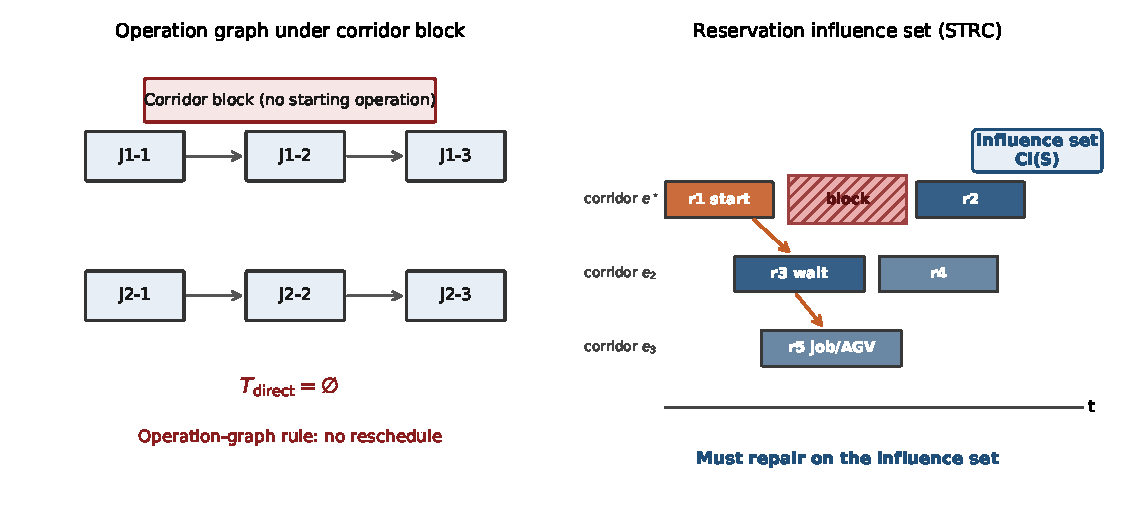
\includegraphics[width=\linewidth]{figures/fig_strc_motivate}
\caption{动机示意。左:走廊阻断不命中任何工序/机器,任务图直接集为空。
右:同一扰动在预约表上产生种子,并沿阻塞与接续关系级联为时空预约闭包。}
\Description{并排两幅图。左幅是任务依赖图,走廊阻断没有命中任何顶点,
直接影响集为空。右幅是同一时刻的走廊预约表,阻断时窗命中若干条预约,
这些预约沿让行边与接续边向外连出一片级联区域。}
\label{fig:motivate}
\end{figure}

\subsection{主张与方法预告}

本文主张三句话。第一,在无冲突柔性作业车间中,扰动影响边界应定义在时空预约图上,
而非仅定义在任务依赖图上。第二,正确的影响对象是\emph{时空预约影响闭包}
(\STRC):以失效预约为种子,沿预约阻塞与调度接续关系取传递闭包;
闭包之外的预约在结构上与种子无依赖,从而「局部」对应一个可检验的对象,
而不是启发式剪枝半径。第三,闭包上的有界修复——释放闭包内预约、外侧冻结、
原车改路,失败则沿工件/车辆链扩大释放——是闭包的应用;升级阶梯中更贵的协调
(换车、改派、改序)可以随后展开,但不是本文创新的挂靠点。

三句话共有一个立场,值得单独点明:\textbf{影响闭包是一次测量,不是一个决策。}
本文不用阻塞关系去\emph{制导}搜索——那样做买的是「改进一个决策」,其收益要经受关键链的
稀释(消去一处走廊等待,往往只是把另一处约束顶成紧约束)。本文用同一份阻塞关系去
\emph{划定}损坏范围——买的是「改进一次测量」,而测量不经受稀释:闭包要么包含了全部必须
释放的预约,要么没有,这与关键链上顶上来的是谁无关。第~\ref{sec:rw_ag}~节用同一句话
区分本文与铁路 alternative graph(那里选弧本身就是决策变量);
第~\ref{sec:relation_static}~节用同一句话说明本文与静态一体化工作对阻塞信息的不同用法。

与「每次扰动都热启动全局重解」相比,\STRC{} 路径回答的是另一侧问题:
在紧响应预算下能否快速恢复可行,并在结构上把修改限制在闭包内。
外侧预约字段的逐条不变是给定边集与预提交成功时的充分条件
(命题~\ref{prop:outside}),不是无条件的恒等式;相对全局重解,
有界修复这条路径改动更少、响应更快。二者的归因不同,第~\ref{sec:cheap}~节把它们分开测过:
响应之快来自「单遍改路、不重开搜索」这一机制形态,而改动之少才是闭包本身兑现的。
实验将表明二者的分工在\emph{响应时间}一侧而不在解质量一侧——闭包修复以极短耗时
恢复可行;全局重解在本文测到的\emph{每一个}挂钟预算点上都取得更优完工时间——
因而正确叙事不是「取代搜索」,而是「测量损坏范围,再决定用多便宜的协调就够」。

\subsection{贡献}
\label{sec:contributions}

按问题层、框架层、机制层、方法层组织,本文贡献如下。

\begin{enumerate}[leftmargin=1.6em,itemsep=0.4em]
\item \textbf{问题层:指认任务图覆盖不到的级联损坏。}
在显式走廊预约下形式化 B 类扰动:按任务图直接集的常规定义,
走廊阻断给出 \(T_{\mathrm{direct}}=\varnothing\);同时证明当预约种子非空时
原排程仍不可行,从而「空影响域 \(\Rightarrow\) 无需重调度」失效。
该缺口既不在常数运输时间模型中可表述,也不在两图合一的模型(如铁路)中出现;
它需要「两张图分立、却只用一张划界」这一特定层级。

\item \textbf{框架层:先测量、再有界协调。}
将动态恢复组织为「闭包划定释放集 \(\rightarrow\) 外侧冻结 \(\rightarrow\)
闭包内最低必要协调」,与「打开种群搜索做全局重解」对照而不混为一谈。
测量优先于协调;修复是框架的第二步而非标题主语。

\item \textbf{机制层:时空预约影响闭包(\STRC)。}
定义种子、依赖边与传递闭包;证明结构闭合性
(闭包外不是闭包内顶点的出边后继),并给出外侧字段不变的\emph{充分条件}
(预提交成功且不扩域时)。此处新的不是让行关系这一对象(见第~\ref{sec:rw_ag}~节),
而是把影响集由算法\emph{过程}的副产品改造成由图结构唯一确定的\emph{对象}:
它可陈述闭合性、可测量规模、可作为不同修复引擎的公共输入。
同引擎消融表明贡献来自边界定义而非某次改路启发式的细节。

\item \textbf{方法层:闭包上的有界恢复与对照协议。}
实现第 1 级改路及失败扩域再修(两者的机制形态均非本文首创,
见第~\ref{sec:rw_aor}、\ref{sec:rw_mapf}~节);在统一无冲突执行器与同挂钟协议下,
对照任务图边界臂与热启动全局重解臂,报告可行性、耗时、预约变动与完工时间,
并给出扰动规模 \(\varphi\) 扫描下的互补关系。

\item \textbf{一张填满的覆盖矩阵,以及一条不利读数。}
在 $50$ 个算例--种子对上,把四类扰动(走廊阻断、路段降速、车辆故障、机械臂故障)
与两种边界定义交叉,给出任务图边界何时为空、闭包相对任务图释放集何时严格更大的
完整读数。同时如实报告:完工时间上有界修复对热启动全局重解全区间劣势、无交叉点;
闭包不最小,覆盖 \(t_{\mathrm{now}}\) 之后活预约的约 \(\ClosureAliveFrac\)。
\end{enumerate}

\subsection{与静态一体化排程工作的关系}
\label{sec:relation_static}

本文可独立阅读。若读者熟悉同一场景下的静态闭环双层排程工作,则二者关系可一句话概括:
\textbf{同一车间、同一预约表;前者用预约表构建排程,本文用预约表定位损坏。}
共享对象是显式路网、走廊独占与半开时窗预约;区别在时机与算法形态——
静态工作在 \(t=0\) 做种群搜索以最小化完工时间,本文在 \(t_{\mathrm{now}}\)
做单解有界恢复以恢复可行并把修改锚定在预约闭包上。

有一处表面上的不一致需要点破。那类静态工作中,\emph{用阻塞关系去制导搜索}
(以「谁挡了谁」的凭证引导邻域算子)往往收效甚微甚至为负;而本文复用的正是同一套阻塞
关系。二者并不矛盾,因为买的东西不同:制导搜索买的是「改进一个决策」,收益要经受关键链
的稀释——消去一处走廊等待,常常只是让另一条约束顶上来成为紧约束,于是净改进被吃掉;
本文买的是「改进一次测量」,而测量不经受稀释——闭包要么含有全部必须释放的预约,要么没有,
这与关键链上顶上来的是谁无关。\textbf{影响闭包是一次测量,不是一个决策};
同一份阻塞信息在这两种用法下有不同的期望回报,恰是这条判据的两侧证据。
独立阅读时,上述静态工作视为相关文献即可。

\subsection{篇章结构}

第~\ref{sec:related_work}~节按「影响边界划在什么对象上」分四层回顾文献,
并划清本文不主张什么。
第~\ref{sec:problem}~节给出系统模型、扰动二分与恢复问题陈述。
第~\ref{sec:strc}~节定义 \STRC{} 并陈述包含性(图~\ref{fig:closure})。
第~\ref{sec:repair}~节描述闭包上的有界修复与扩域策略(图~\ref{fig:framework})。
第~\ref{sec:experiments}~节报告实验,并以案例甘特衔接统计与时间轴。
第~\ref{sec:conclusion}~节总结,并分节给出局限与后续工作。

%% =====================================================================
\section{相关工作}
\label{sec:related_work}
%% =====================================================================

%% 本节 2026-08-16 整体重写。原稿只引 vieira2003 / ouelhadj2009 两篇综述就断言
%% 「影响域一直划在任务图上」,这对一个针对整支文献的判断是不够的:R1 会被读成
%% 稻草人。重写按「边界划在什么对象上」分四层,前三层都是本文\emph{不}主张新颖性
%% 的地方,第四层才是本文的位置。三条禁语(见 2.5)由此固定下来。

影响边界的划定并非新问题;真正区分各支文献的是\emph{边界划在什么对象上}。
据此本节分四层:①~任务图或时间轴(2.1);②~让行图,但与任务图合为一张(2.2);
③~只有让行图而无任务图(2.3);④~两张图并存,却仍只用任务图划界(2.4)——
最后一层是本文的位置。表~\ref{tab:position} 汇总。

\subsection{任务图与时间轴上的影响边界}
\label{sec:rw_aor}

在任务依赖图上划界的原型是\textbf{受影响工序重调度}(Affected Operations
Rescheduling, AOR)。Li 等人~\cite{li1993heuristic} 以调度二叉树与 MRP 的净改变
概念只修订「需要修订的工序」;Abumaizar 与 Svestka~\cite{abumaizar1997rescheduling}
给出完整的 AOR 算法——只重排受扰动\emph{直接或间接}影响的工序,其余保持原次序,
并以效率与稳定性两个维度同完全重调度、右移重调度对比;Subramaniam 与
Raheja~\cite{subramaniam2003maor} 的 mAOR 把它从单一机器故障推广到插单、工时偏差、
订单取消等多种扰动。\textbf{本文的 R1 对照臂就是 AOR:}以失效工序为种子,沿工件后继
与机器链扩张,再只重排影响域内的部分。把它写成对照不是因为它弱,而是因为它是这一支的
标准做法,且其种子定义直接决定了本文要检验的那件事。

沿\emph{时间轴}划界是同样成熟的另一条路。match-up 调度~\cite{bean1991matchup}
在扰动点之后选一个匹配时刻,只重排两者之间的部分,并给出该策略最优的条件;
Aktürk 与 Görgülü~\cite{akturk1999matchup} 用反馈机制确定匹配点。
Local Rescheduling~\cite{kuster2007local} 则把时间窗\emph{增量式扩张}直到找到可行解,
并明确指出 AOR 与 match-up 都绑定在生产特有的问题结构上。
右移重调度则响应最快而不需要任何边界:它把未完成的部分整体后推,不判定谁受影响。
近期一项考虑 AGV 与执行期故障的工作仍把「完全重调度 / 部分重调度 / 右移」并列为同一组
取舍,并指出右移保住了稳定性却让出了优化空间~\cite{tang2026dynamic}。
本文把它实现为对照臂之一(第~\ref{sec:cheap}~节),因为它正是「不划边界」这一端点。
滚动时域与分解式方法在规模与质量之间折中~\cite{zeitrag2025novel,zhao2019decomposition};
两篇综述系统梳理了完全重调度与修复式重调度的取舍~\cite{vieira2003rescheduling,ouelhadj2009survey}。

这一层给出两点纪律。其一,\textbf{「应当划一个边界」不是本文的主张},它至少有三十年历史;
本文能主张的只是边界该划在\emph{哪个图}上。其二,\textbf{「失败后扩大释放域」不是本文的机制创新}
——LRS 已是沿时间窗扩张,本文第~\ref{sec:scope_escalation}~节沿依赖边扩张只是同一思路
换了扩张方向。这一层的共同隐含前提是:扰动首先是一个任务事件。一旦扰动只使走廊时窗失效
而不改指派,该前提不再成立,任务图种子可以为空,而排程已不可行。

\subsection{让行图已有先例:alternative graph 与铁路实时重调度}
\label{sec:rw_ag}

「谁在排他资源上先于谁」这一关系被显式建成图,在铁路调度中已有二十余年历史。
Mascis 与 Pacciarelli~\cite{mascis2002alternative} 的 \emph{alternative graph}
把析取图推广为:顶点是作业在\emph{闭塞区段}上的占用,固定弧表达路径先后,
成对的 alternative arc 表达「谁先通过该区段」。D'Ariano 等人~\cite{dariano2007branch}
以该模型做实时列车重调度,在扰动后重算无冲突时刻表并最小化与原时刻表的偏离。
\textbf{本文的让行边与 alternative arc 是同一个对象},必须先承认这一点。
两处区别决定了本文仍然成立:

\begin{itemize}[leftmargin=1.5em,itemsep=0.25em]
\item \textbf{用途不同:选弧 vs 取闭包。} 在 alternative graph 里,弧的\emph{选择本身是
决策变量}——求解即选一组弧使图无正环且目标最优。本文\emph{不选择弧}:让行边由已经落盘的
那份排程唯一确定,本文在这一\emph{既定选择}之上取传递闭包,回答的是另一个问题——
扰动之后哪些承诺必须作废。用一句话说,\textbf{影响闭包是一次测量,不是一个决策}。
\item \textbf{模型层级不同,而这个差别正是本文问题的来源。} 在铁路模型里闭塞区段\emph{就是}
机器,任务图与让行图合为一张;因此「区段阻断」在那里天然属于 A 类,不存在任务图看不见的
问题。本文的缺口只在\emph{两张图分立}的模型里存在。这既是对该文献的礼让,
也是本文问题得以成立的前提。
\end{itemize}

\subsection{无任务图的局部重规划:MAPF 的 Replan Affected}
\label{sec:rw_mapf}

在多智能体路径规划中,「只为受影响者重规划、其余视作动态障碍」已是标准做法。
Švancara 等人~\cite{svancara2019online} 在在线 MAPF 中明确给出 Replan All /
Replan Single / \textbf{Replan Affected} 三档,并以在线独立性检测确定受影响集合;
Malka 等人~\cite{malka2024online} 在地图不准确的设定下同样「只为受观测变化影响的
智能体重规划」。无冲突路径规划把时空占用作为一等约束,但任务集合与端点通常由外部
给定~\cite{zhang2024guidance}。

因此\textbf{「闭包内重规划 + 闭包外冻结」这一机制形态不是本文的创新},本文不作此声称。
MAPF 之所以不会遇到本文的问题,是因为它\emph{根本没有任务图}:任务外生,不存在
「任务图看不见」这回事。它与本文的区别也不在机制,而在影响集的性质——
独立性检测的输出是算法过程的副产品,随实现与终止条件而变;闭包是由图结构唯一确定的
对象,可陈述闭合性、可测量规模、可作为不同修复引擎的公共输入
(第~\ref{sec:containment}~节)。

\subsection{两张图并存的场合:考虑运输的柔性作业车间}
\label{sec:rw_position}

考虑运输车辆的柔性作业车间调度已有系统综述~\cite{xin2025review}。
近期组合优化工作仍普遍把行驶时间取为按位置索引的常数矩阵,
并在此之上发展约束规划、元启发式与知识引导搜索~\cite{meng2025cp,qin2026knowledge,fu2025integrated}。
在该建模约定下,车辆互不占用同一时空资源,延误不是一车施加给另一车的量;
走廊阻断这类事件甚至没有对应的模型对象。因此,「任务图覆盖不到的预约级联」
在常数矩阵文献中既不会被提出,也无法被检验——这不是那些工作的缺陷,
而是本文问题附着于另一建模层级的原因。

一旦下层改用显式走廊预约,两张图就同时存在了。制造场景中的拥堵感知派车以局部密度等
代理量驱动选车,而不回头改机器指派~\cite{kim2026congestion}。把柔性指派与无冲突运输
真正耦合的工作相对较少:van Os 与 Basten~\cite{vanos2026exact} 形式化了带无冲突运输
约束的柔性作业车间调度问题,并以分解方法给出可证最优基准;两阶段方案先固定排产再消解
车辆冲突~\cite{sun2023integrated};亦有以学习层排产、路径层消冲突并以有限反馈连接的
框架~\cite{li2026framework}。这些工作主要回答静态或准静态下如何\emph{构建}可行且高质量
的一体化排程。

\textbf{把预约表与执行期扰动同时纳入的工作目前还没有,而两侧各自为什么没跨过来,
文献里写在明处。} 持有预约表的一侧把执行期故障排除在模型之外:Sun 等~\cite{sun2023integrated}
以时间窗 Dijkstra 消解车辆冲突,却在假设中声明车辆「始终可用,不考虑其故障与充电」,
并在结尾把设备维护与故障列为后续研究。反过来,在柔性作业车间上真正处理执行期扰动的
AGV 工作,其影响边界一律落在任务对象上:Zhang 等~\cite{zhang2023energy} 处理机器故障与
插单,恢复范围是「故障之后尚未加工的工序整体重排」——一个纯粹的工序集合;Tang
等~\cite{tang2026dynamic} 按扰动传播把工序与配送任务分为保留、继续、重构三类,边界同样
划在任务与配送任务上。而这两篇之所以能一致地这样划,恰恰因为它们\emph{不}持有预约表:
前者在模型假设中明写「忽略 AGV 之间的碰撞」。

于是缺口的性质不是「某篇工作用错了边界」,而是结构性的:\textbf{工序级边界成立的前提正是
没有预约表,而现有的预约表设定又恰好把执行期扰动排除在外,两个条件至今没有同时松开。}
一旦松开——而上述静态一体化工作都把执行期扰动列为下一步——可继承的现成边界只有第
2.1 节那一套,它对不改动任何工序指派的扰动会给出空的影响集(第~\ref{sec:e1}~节实测
\PassMiss)。本文要处理的就是这一格。

\subsection{本文定位,以及本文不主张什么}
\label{sec:rw_claim}

\begin{table*}[t]
\centering
\caption{按「影响边界划在什么对象上」定位。最后一列是本文与该层的关系;
前三层本文均\emph{不}主张新颖性。}
\label{tab:position}
\small
\begin{tabular}{@{}p{0.155\linewidth}p{0.195\linewidth}p{0.135\linewidth}p{0.125\linewidth}p{0.275\linewidth}@{}}
\toprule
\textbf{层} & \textbf{代表工作} & \textbf{边界划在} & \textbf{有任务图?} & \textbf{与本文的关系} \\
\midrule
① 任务图 / 时间轴 &
AOR~\cite{li1993heuristic,abumaizar1997rescheduling,subramaniam2003maor};
match-up~\cite{bean1991matchup,akturk1999matchup}; LRS~\cite{kuster2007local} &
工序集合 / 时间窗 & 有 &
\textbf{R1 即 AOR。} 边界划定与失败扩域皆非本文首创 \\
\addlinespace[2pt]
② 让行图,两图合一 &
alternative graph~\cite{mascis2002alternative}; 铁路实时重调度~\cite{dariano2007branch} &
闭塞区段占用 & 有,但\emph{与让行图同一张} &
让行边同源。区别:选弧(决策)与取闭包(测量);且区段即机器,故无本文缺口 \\
\addlinespace[2pt]
③ 让行图,无任务图 &
Online MAPF 的 Replan Affected~\cite{svancara2019online,malka2024online};
LMAPF~\cite{zhang2024guidance} &
受影响智能体 & 无(任务外生) &
「局部重规划 + 外侧冻结」为其标准做法,本文不作机制创新;
区别在影响集是\emph{过程}还是\emph{对象} \\
\addlinespace[2pt]
④ 两图并存 &
常数矩阵 FJSP--AGV~\cite{xin2025review,meng2025cp,qin2026knowledge,fu2025integrated};
一体化排程~\cite{vanos2026exact,sun2023integrated,li2026framework};
执行期扰动~\cite{zhang2023energy,tang2026dynamic} &
工序集合 & 有,且另有预约表 &
\textbf{本文的位置。} 两图并存与执行期扰动至今未同时出现;
一旦并置,继承自①的边界与损坏的载体错位 \\
\bottomrule
\end{tabular}
\end{table*}

综上,本文的主张必须收窄到第 ④ 层:\emph{在同时持有任务依赖图与显式走廊预约表的
这一支调度文献中},可继承的影响边界仍是任务图那一套,而它对 B 类扰动系统性失效。
写成对「局部重调度文献」的全称否定是不成立的——第 ② 层不会犯这个错(两图合一),
第 ③ 层不可能犯(没有任务图),缺口只在第 ④ 层这个特定的模型层级上存在。
也\emph{不}应写成「已有工作在这一格上划错了边界」:如上节所引,这一格里两图并存与
执行期扰动至今没有同时出现过,因此本文指认的是一个\emph{在两者并置时必然出现}的失效,
而不是对某篇具体工作的纠错。相应地,R1 对照臂复现的是第 ① 层的标准做法,
不代表任何一篇第 ④ 层工作的实际选择。

相应地,本文\textbf{不}主张以下三件事,后文亦不再以创新的口吻提及:
(i)~「只重规划受影响者、其余冻结为障碍」这一机制形态(第 ③ 层已有);
(ii)~「单次修复失败后扩大释放域」(LRS 已有,只是沿时间窗而非沿依赖边);
(iii)~「用让行关系组织冲突」这一建模对象(alternative graph 已有)。
本文主张的是:该边界应\emph{改画在预约图上},并且这一改画可以被定义成一个
有闭合性、可测量的对象,而不是又一条启发式规则。

%% =====================================================================
\section{问题描述}
\label{sec:problem}
%% =====================================================================

\subsection{系统设定与记号}
\label{sec:system_brief}

我们采用带无冲突运输约束的柔性作业车间设定~\cite{vanos2026exact} 的执行期版本,
记号与静态闭环解码器对齐,此处只保留后文需要的对象。

车间路由图 \(G=(V,E)\) 强连通;每条走廊 \(e\in E\) 为排他资源,通行时间 \(\tau_e\) 已知。
占用记为半开区间。\(n\) 个工件、机器集合 \(M\)、车队 \(K=\{1,\ldots,N_A\}\)。
工序 \(O_{ji}\) 的候选机器集为 \(\Omega_{ji}\subseteq M\)。
一份完整排程
\[
\mathcal{S}=(x,\,\pi,\,y,\,R)
\]
包含机器指派 \(x\)、工序扫描序 \(\pi\)、车辆指派 \(y\),以及预约表
\[
R=\bigl\{\,r=(e,\,[t^s,t^e),\,k,\,u)\,\bigr\},
\]
其中 \(k\in K\) 为车辆,\(u\) 为任务标签(空载/满载段)。
路径只占用 \(R\) 报告为空闲的时窗,从而构造性保持无冲突。

任务依赖图 \(G_T=(T_T,E_T)\) 以工序(或工序级任务 id)为顶点,
边为工件前后约束;它\emph{不}包含走廊占用之间的阻塞边。
预约依赖图 \(G_R=(R,E_R)\) 的顶点为 \(R\) 中的预约记录,边集见第~\ref{sec:strc}~节。

\begin{table}[t]
\centering
\caption{本文常用记号}
\label{tab:notation}
\small
\begin{tabular}{@{}ll@{}}
\toprule
\textbf{符号} & \textbf{含义} \\
\midrule
\(G=(V,E)\) & 走廊路网 \\
\(R\) & 走廊预约表(半开占用区间集合) \\
\(G_T\) / \(G_R\) & 任务依赖图 / 预约依赖图 \\
\(\mathcal{S}^0,\mathcal{S}'\) & 扰动前排程、恢复后排程 \\
\(\mathcal{D},\,t_{\mathrm{now}}\) & 扰动事件、发生(决策)时刻 \\
\(T_{\mathrm{direct}},\,T_{\mathrm{impact}}\) & 任务图直接/ \(\theta\)-跳影响域 \\
\(\mathrm{Seeds}(\mathcal{D})\) & 与扰动重叠的预约种子 \\
\(\mathrm{Cl}(\cdot)\) & 时空预约影响闭包(\STRC) \\
\(\varphi\) & 受扰未来工序比例(规模扫描) \\
\bottomrule
\end{tabular}
\end{table}

\subsection{假设:从静态完备到执行期扰动}
\label{sec:assumptions}

静态构建阶段可沿用「信息完备、构造性可行、计划期内无故障」等约定。
本文打开执行期扰动,其余物理假设保持不变以便归因:

\begin{enumerate}[label=\textbf{A\arabic*.},leftmargin=*,topsep=2pt,itemsep=2pt]
\item \textbf{初始排程可行。} \(\mathcal{S}^0\) 在扰动前通过无冲突校验;预约表与工序时间表一致。
\item \textbf{扰动在 \(t_{\mathrm{now}}\) 被观测。} 已完成占用不回溯修改;只重协调
\(t_{\mathrm{end}}>t_{\mathrm{now}}\) 的未来预约与未完工工序。
\item \textbf{走廊仍为排他半开资源。} 阻断以附加占用(或禁行窗)注入路由层。
\item \textbf{缓冲与同构车队等与静态设定一致。} 有限缓冲、充电等仍不建模。
\item \textbf{允许的恢复动作。} 本文实现级默认:保持原机器指派与扫描序,允许改路;
失败时扩大释放集。换车/改派/改序留作升级阶梯的后续级,实验中全局重解对照臂可改染色体。
\end{enumerate}

\subsection{扰动二分}
\label{sec:disturbance_classes}

\begin{definition}[A/B 类扰动]
\label{def:ab}
若扰动直接使某些工序的指派或\emph{可执行性}失效(机械臂故障、显著工时偏差、插单、
车辆故障等),称其为 \textbf{A 类};若扰动只使某些走廊时窗不可用、而不使任何工序
不可执行(走廊阻断、路段降速等),称其为 \textbf{B 类}。
\end{definition}

\begin{remark}[车辆故障为何属于 A 类]
\label{rem:agv_class}
车辆故障不改动任何工序的机器指派,乍看应与走廊阻断同类。但定义~\ref{def:ab} 的判据是
\emph{可执行性}而非指派:一辆车抛锚后,它承运的那些工序在原计划下无法开工,
故经「车辆\(\to\)所承运工序」的映射,任务图上留有非空种子。这一归类是保守的,
它把一类边缘情形判给了对本文\emph{不利}的一侧——A 类是任务图边界能看见的那一类。
需要指出,只有当重调度框架维护了车--任务映射时该种子才非空;若框架只跟踪工序与机器
(AOR 的常见实现即如此),车辆故障同样会漏报。本文不依赖这一点立论,
第~\ref{sec:e6}~节按维护了该映射的强口径报告 A 类读数。
\end{remark}

\begin{definition}[任务图直接集与影响域]
\label{def:task_impact}
对扰动 \(\mathcal{D}\),令 \(T_{\mathrm{direct}}(\mathcal{D})\) 为被故障智能体或失效工序
直接命中的任务 id 集合。对 B 类走廊扰动约定 \(T_{\mathrm{direct}}=\varnothing\)。
在 \(G_T\) 上从 \(T_{\mathrm{direct}}\) 出发做深度至多 \(\theta\) 的扩张,记为
\(T_{\mathrm{impact}}(\mathcal{D},\theta)\)。
\end{definition}

\begin{definition}[预约种子]
\label{def:seeds}
种子集 \(\mathrm{Seeds}(\mathcal{D})\subseteq R\) 按扰动类型给出,一律只取
\(r.t^e>t_{\mathrm{now}}\) 的预约。
\begin{enumerate}[label=(\alph*),leftmargin=1.6em,itemsep=0.15em]
\item \textbf{走廊阻断/降速} \(\mathcal{D}=(e,[t_a,t_b))\):
\(\{\,r:\ r.e=e,\ [r.t^s,r.t^e)\cap[t_a,t_b)\neq\varnothing\,\}\)。
多微阻断时取各窗种子之并。两者共用这条规则(降速在当前实现中按整段不可用处理),
故它们给出同一个种子集——第~\ref{sec:e6}~节据此说明为何不把二者算作两次独立验证。
\item \textbf{车辆故障} \(\mathcal{D}=(k)\):该车在 \(t_{\mathrm{now}}\) 之后的全部预约
\(\{\,r:\ r.k=k\,\}\)。
\item \textbf{机械臂故障} \(\mathcal{D}=(m,F)\),\(F\) 为该机上尚未完工的工序:
对每个工件取 \(F\) 中最小工序号 \(i_{\min}(j)\),种子为各工件自该工序起(含)的全部
未来预约。之所以沿工件链向后取而不只取该工序自身,是因为进站运输可能已在
\(t_{\mathrm{now}}\) 前结束,若只取自身,闭包会短于任务图影响域,对照即不公平。
\end{enumerate}
\end{definition}

\begin{prop}[B 类上的任务图空洞]
\label{prop:miss}
设 \(\mathcal{D}\) 为走廊阻断。若采用定义~\ref{def:task_impact} 对 B 类的约定,则
\(T_{\mathrm{direct}}(\mathcal{D})=\varnothing\),从而对任意有限 \(\theta\ge 0\) 有
\(T_{\mathrm{impact}}(\mathcal{D},\theta)=\varnothing\)。
若此外 \(\mathrm{Seeds}(\mathcal{D})\neq\varnothing\),则 \(\mathcal{S}^0\) 在 \(\mathcal{D}\) 下不可行。
\end{prop}

\begin{proof}
由定义~\ref{def:task_impact},走廊阻断不命中任何故障智能体或失效工序,故
\(T_{\mathrm{direct}}=\varnothing\)。\(\theta\)-跳扩张的起点为空,故
\(T_{\mathrm{impact}}=\varnothing\)。
若存在 \(r\in\mathrm{Seeds}(\mathcal{D})\),则 \(r\) 的占用区间与禁行窗相交。
将 \(\mathcal{D}\) 解释为该走廊上的强制占用后,\(r\) 与禁行窗在同一排他资源上时间重叠,
违背半开时窗无冲突条件,故 \(\mathcal{S}^0\) 不可行。
\end{proof}

命题~\ref{prop:miss} 即问题层的一击反例。前半句是任务图直接集对 B 类的约定推论
(指出任务图\emph{表示}覆盖不到走廊事件);非平凡的是后半句——种子非空时排程已不可行,
因而「空影响域 \(\Rightarrow\) 无需重调度」在无冲突设定下不成立。
该反例不依赖任何修复算法;实验第~\ref{sec:experiments}~节给出算例规模。

\subsection{恢复问题}
\label{sec:recovery_problem}

\begin{problem}[预约表感知的有界恢复]
\label{prob:recovery}
给定可行排程 \(\mathcal{S}^0\)、扰动 \(\mathcal{D}\) 与时刻 \(t_{\mathrm{now}}\),
求 \(\mathcal{S}'\),使得:
(i)~\(\mathcal{S}'\) 在 \(\mathcal{D}\) 下通过无冲突校验;
(ii)~未释放预约的字段尽可能与 \(\mathcal{S}^0\) 一致;
(iii)~墙钟响应时间受预算约束。
次级目标为完工时间 \(C_{\max}(\mathcal{S}')\)。
\end{problem}

框架层将求解拆为两步:\textbf{测量}——计算释放集 \(U\subseteq R\);
\textbf{协调}——仅对 \(U\) 内运输重规划,外侧冻结。
本文测量用 \(\mathrm{Cl}(\mathrm{Seeds})\);对照测量用任务图影响域诱导的预约子集。

%% =====================================================================
\section{时空预约影响闭包}
\label{sec:strc}
%% =====================================================================

\subsection{预约依赖边}
\label{sec:closure_def}

\begin{definition}[预约依赖图]
\label{def:dep}
顶点为 \(R\) 中预约。有向边 \(r\to r'\) 表示「\(r\) 失效可能迫使 \(r'\) 重规划」,包括:
\begin{enumerate}[leftmargin=1.4em,itemsep=0.15em]
\item \textbf{让行边:} 同走廊、异车、时间重叠,且先进入者指向后进入者;
\item \textbf{同车后继:} 同一车辆按时间序相邻的两条预约;
\item \textbf{同工件后继:} 同一工件工序 \(i\) 的预约指向工序 \(i+1\) 的预约;
\item \textbf{同机后继:} 同一机器时间轴上相邻两道工序所诱导的预约之间的边。
\end{enumerate}
由此得到 \(G_R=(R,E_R)\)。
\end{definition}

\begin{definition}[\STRC{}]
\label{def:strc}
对种子集 \(S\subseteq R\)、视界 \(H\) 与时刻 \(t_{\mathrm{now}}\),
记活预约为
\[
R^{\circ}=\bigl\{\,r\in R:\ r.t^e>t_{\mathrm{now}},\ r.t^s<H\,\bigr\},
\]
并令 \(G_R^\circ\) 为 \(G_R\) 在 \(R^{\circ}\) 上的诱导子图。
时空预约影响闭包定义为
\[
\mathrm{Cl}(S)
=\bigl\{\,v\in R^{\circ}:\
\exists\,s\in S\cap R^{\circ}\ \text{使}\ s\!\to^*\!v\ \text{于}\ G_R^\circ\,\bigr\},
\]
即从活种子出发沿出边可达的全部活顶点(含种子自身)。
若以邻接表表示 \(G_R^\circ\),则可用队列在 \(O(|R^{\circ}|+|E_R^{\circ}|)\) 时间内算出。
\end{definition}

图~\ref{fig:closure} 给出玩具示意:(a) 阻断窗与种子;(b) 依赖边与闭包外壳,
闭包外顶点不是闭包内顶点的出边后继(命题~\ref{prop:struct})。

\begin{figure}[t]
\centering
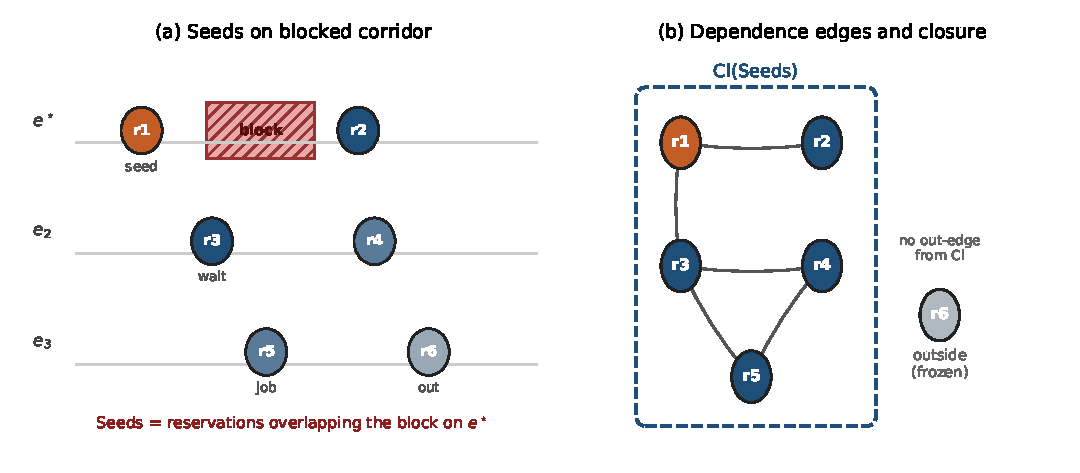
\includegraphics[width=\linewidth]{figures/fig_strc_closure}
\caption{时空预约闭包构造示意。
(a)~走廊阻断命中种子预约;
(b)~沿让行/接续边取传递闭包 \(\mathrm{Cl}(\mathrm{Seeds})\),外侧预约定向冻结。}
\Description{两小幅示意图。(a) 时空图上一段阻断窗覆盖若干条预约,
这些预约被标为种子。(b) 从种子沿有向依赖边做传递闭包,得到一圈闭包外壳;
外壳之外的预约没有来自壳内的入边,被标注为冻结。}
\label{fig:closure}
\end{figure}

对照的任务图边界臂(记 R1)将 \(T_{\mathrm{impact}}\) 映射为预约释放集:
凡任务标签属于影响域且 \(t^e>t_{\mathrm{now}}\) 的预约。
由命题~\ref{prop:miss},B 类上该集合为空;闭包臂(记 R2)取 \(U=\mathrm{Cl}(\mathrm{Seeds})\)。

\subsection{包含性}
\label{sec:containment}

\begin{prop}[结构闭合性]
\label{prop:struct}
对任意 \(S\subseteq R\),在 \(G_R^\circ\) 中不存在边
\(u\to v\) 满足 \(u\in\mathrm{Cl}(S)\) 且 \(v\in R^{\circ}\setminus\mathrm{Cl}(S)\)。
因而,从 \(\mathrm{Cl}(S)\) 出发沿出边无法到达闭包外的活预约。
\end{prop}

\begin{proof}
若存在这样的边 \(u\to v\),则由 \(u\in\mathrm{Cl}(S)\) 知存在活种子 \(s\) 使
\(s\to^* u\)。拼接 \(u\to v\) 得 \(s\to^* v\),故按定义~\ref{def:strc} 应有
\(v\in\mathrm{Cl}(S)\),矛盾。
\end{proof}

命题~\ref{prop:struct} 说明「局部」对应一个图论闭合对象:闭包外顶点不是任何
闭包内顶点的直接后继。它\emph{不}声称 \(G_R\) 已枚举物理世界中一切可能耦合——
边集是建模选择;一旦边集固定,闭合性就是定义的推论,而不是启发式半径。

\begin{remark}[本文不作最小性主张]
\label{rem:minimality}
闭合性说的是闭包\emph{足够大},没有说它\emph{不过大}。二者是两个方向,后者本文不主张,
理由有三,按分量排列。

其一,\textbf{最小释放集的定义依赖于修复引擎,而闭包刻意不依赖}。称释放集 \(U\) 为最小,
须指明「在何种修复能力下 \(U\) 足以恢复可行」。允许改派与改序时的最小 \(U\),
与只允许改路时的最小 \(U\) 不是同一个集合。闭包由 \(G_R\) 唯一确定,与引擎无关——
这正是它能作为不同引擎公共输入的原因,也是它无法同时具备最小性的原因。

其二,\textbf{四类边是充分方向的过近似}。让行边按「同走廊、异车、时间重叠」建立,
只要两条预约在时间上重叠即连边,而不判断后者是否\emph{真的}只能靠等待前者通过——
若走廊网络在该处另有旁路,后者改道即可,本不必进入释放集。同理,同车后继边把一辆车
在 \(t_{\mathrm{now}}\) 之后的整条链连通,而一次早期延误未必传得到链尾。
这两处都会使闭包严格大于必要。

其三,\textbf{实测证实闭包确实不小}。第~\ref{sec:e6}~节报告,走廊阻断下闭包平均覆盖
\(t_{\mathrm{now}}\) 之后活预约的约 \(90\%\);换言之,相对「释放全部未来预约」这一平凡
上界,闭包省下的不足一成。有界修复真正省下的是\emph{不动过去}与\emph{不重开搜索},
而不是把未来切得很小。这一点在第~\ref{sec:e5}~节与局限一节中再次点明,
不应被「局部」「有界」这两个词误导。

不过「省下的不足一成」是释放集的\emph{规模}之比,不等于闭包的价值之比:
第~\ref{sec:cheap}~节把那个平凡上界作为一条独立对照臂(RA)实测后发现,正是这不足一成的
差别,把改动比例从 \ResFracAllFuture\ 降到 \ResFracCheapRtwo(逐格 \RAStabWTL,
\(p=\RAStabP\)),而耗时与完工时间几乎不变。所以本注否证的是「闭包很小」,
不是「闭包无用」——这两句话此前容易被读混。

因此本文的定位是:闭包给出一个由结构唯一确定、可复现、\emph{足以}恢复可行的释放集,
并附带闭合性保证;逼近最小释放集是另一个问题,列为后续工作
(第~\ref{sec:future}~节)。
\end{remark}

\begin{prop}[外侧字段不变的充分条件]
\label{prop:outside}
设释放集 \(U=\mathrm{Cl}(S)\),并设第 1 级协调按第~\ref{sec:level1}~节执行:
(i)~禁行窗已写入路由层;(ii)~对每个 \(r\in R^{\circ}\setminus U\),将其原字段
\((e,[t^s,t^e),k)\) 预提交到新预约表且预提交成功;
(iii)~仅对 \(U\) 内运输调用路由器生成新占用;(iv)~最终排程通过无冲突校验。
则在恢复后的预约表 \(R'\) 中,每个外侧任务标签对应的占用字段与 \(\mathcal{S}^0\) 一致。
\end{prop}

\begin{proof}
由 (ii),外侧预约在重放开始前已按其原区间写入新表,且未与禁行窗冲突
(否则预提交失败)。步骤 (iii) 只为 \(U\) 内任务提交新占用,不删除或改写已提交的
外侧区间。因此,对外侧任务标签,新表中的 \((e,[t^s,t^e),k)\) 与预提交值相同,
亦即与 \(\mathcal{S}^0\) 相同。校验通过仅排除新占用与既有占用冲突,不改变已提交字段。
\end{proof}

\begin{remark}[前提 (ii) 与 (iii) 各自会怎样失效]
\label{rem:precommit}
若预提交因「外侧与禁行窗重叠」失败,则 \(S\) 未能覆盖全部直接命中预约,闭包种子不完备。
若协调因运输--工序衔接失败而触发第~\ref{sec:scope_escalation}~节扩域,则新的释放集
\(U'\supsetneq U\),命题~\ref{prop:outside} 只对最终未释放的外侧成立。
扩域以可行性优先于最小扰动,实验中单独报告。
还有一种失效不在命题的可控范围内,但在实现上极易发生:前提 (iii) 要求路由器\emph{只}
为 \(U\) 内的运输生成新占用。若实现以比预约更粗的单位(例如整道运输、整个工序)决定
是否重规划,则 \(U\) 外的占用会被顺带改写,命题的结论随之落空——不是命题错了,
而是前提没被满足。注~\ref{rem:e2b_history} 记录了本文在这一点上踩过的坑。
\end{remark}

\subsection{结构可预测性}
\label{sec:structure}

闭包规模不是可调参数,而是由排程与网络结构决定的量:它随算例规模稳定上升
(第~\ref{sec:e1}~节)。这使「局部」成为一个可以测量的量,而不是一个人为设定的半径。

至于\emph{哪种}结构会产生更大的闭包,本文的答案是否定的,而且否定得比「没测出来」更明确:
\textbf{闭包规模不由装卸点处的静态割决定}。在自建的同规模布局上,不同边界阻断协议下的
相对闭包或落在很窄的带内、或虽有方向但逐种子取值高度重叠;换用一批不由本文设计的路网后,
装卸点最小割与漏斗占比\emph{取值恒定},而闭包占比在路网不变、仅改机器落位时即大幅移动
——一个恒定的量不可能解释一个变动的量(第~\ref{sec:e4}~节)。
须同时说明这条否定的适用范围:它否的是「静态割能解释闭包规模」这一具体命题,
\emph{不是}「结构与闭包规模无关」。可得的公开路网数量有限,后者尚不可判。
本文因此不把闭包规模的结构可预测性列为贡献;下一个候选刻画应是随排程而变的量,
而非纯拓扑量(第~\ref{sec:future}~节)。

%% =====================================================================
\section{闭包上的有界修复}
\label{sec:repair}
%% =====================================================================

图~\ref{fig:framework} 总览本文流程:先以 \STRC{} \emph{测量}释放集,
再在闭包上做第 1 级有界协调;失败则扩域重试。
对照臂 R1 仅替换释放集来源,R0+ 则打开热启动搜索——同一无冲突执行器上归因。

\begin{figure}[t]
\centering
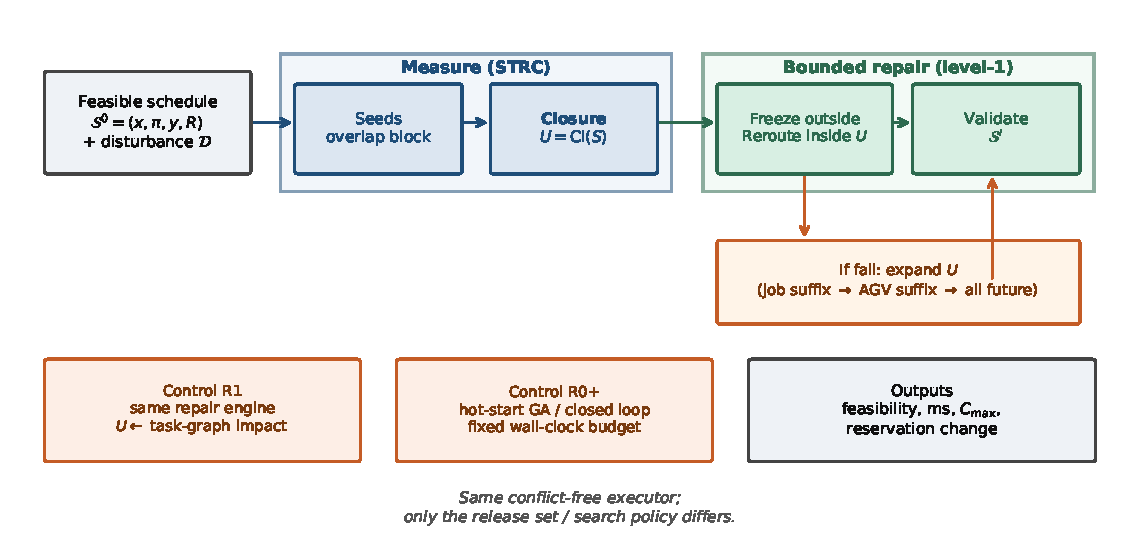
\includegraphics[width=\linewidth]{figures/fig_strc_framework}
\caption{\STRC{} 有界恢复框架。
上排:扰动下由种子取闭包并改路;中排:失败扩域;
下排:R1(任务图边界)与 R0+(热启动重解)对照及输出指标。}
\Description{三排流程图。上排:扰动进入后由种子取闭包,释放闭包内预约、
冻结闭包外预约,然后原车改路。中排:改路失败时按工件后缀、同车后缀、
全部未来的顺序扩大释放集并重试。下排:两条对照臂,R1 用任务图影响域替换释放集,
R0+ 用热启动全局搜索;三条路径汇入同一组输出指标。}
\label{fig:framework}
\end{figure}

\subsection{释放、冻结与第 1 级改路}
\label{sec:level1}

给定释放集 \(U\),第 1 级协调保持原车辆指派与机器指派,按原扫描序重放:

\begin{enumerate}[leftmargin=1.4em,itemsep=0.2em]
\item 将扰动禁行窗写入路由层;
\item 对 \(r\notin U\) 的未来预约预提交到预约表(外侧冻结);若外侧已与禁行窗冲突,
    则闭包漏网,直接失败;
\item 对释放集内运输:原车在当前表上重规划空载/满载段并提交;
\item 推进机器空闲时刻与工件就绪时刻;以独立校验器验收,并禁止修复后占用仍落入禁行窗。
\end{enumerate}

该级不打开种群搜索。同引擎消融(E3)固定上述步骤,仅替换 \(U\) 来自 R1 或 R2,
用以把贡献归因于边界定义。

\subsection{失败扩域再修}
\label{sec:scope_escalation}

\textbf{先声明:扩域机制本身不是本文首创。} Local Rescheduling~\cite{kuster2007local}
已给出「增量式扩张时间窗直至可行」的做法,AOR 的间接影响传播亦是一种扩张
(第~\ref{sec:rw_aor}~节)。本文的差别只在扩张\emph{沿什么走}——沿依赖边而非沿时间窗——
这不足以单独作为贡献。本节的作用是把闭包路径补成一个完整可用的流程,
并在第~\ref{sec:protocol}~节交代它为何必须在边界消融中关闭。

当外侧冻结过紧时,第 1 级可能因运输--工序衔接等校验失败。
此时不立刻求助于全局 GA,而按下列顺序扩大 \(U\) 并重试同一引擎:
(i)~并入释放集内各工序的同工件后缀未来预约;
(ii)~并入涉及车辆的同车后缀;
(iii)~必要时释放全部未来预约。
扩域仍是确定性单遍协调。实验表明扩域可将可行率拉至全样本,耗时仍保持在毫秒至十余
毫秒量级(第~\ref{sec:experiments}~节)。需要说明的是,耗时随扰动比例 \(\varphi\)
并不单调(表~\ref{tab:scale}):比例小时初始闭包偏紧、冻结偏多,扩域更常被触发;
比例大时初始释放已较松、往往一轮成功,但单轮要重规划的运输更多。
两种效应方向相反,故本文不宣称耗时随 \(\varphi\) 有可预测的走向,只宣称它不随
\(\varphi\) 崩溃。

\subsection{与全局重解的对照}
\label{sec:vs_r0}

对照臂在相同禁行约束下,以 \(\mathcal{S}^0\) 的染色体热启动做固定挂钟预算的闭环搜索
(记 R0+)。它可改派与改序,因而更可能改善 \(C_{\max}\),但耗时由预算决定。
对照取热启动而非冷启动,是因为对照必须取强者:冷启动会白白丢掉原解携带的全部信息,
赢它不说明问题。

角色分工是:\STRC{} 路径优先可行性与响应时间,并在结构上限制释放集;R0+ 优先完工时间。
需要预先说明这个「分工」的确切含义——它\emph{不}是指存在某个预算区间使闭包路径的
\(C_{\max}\) 更优。第~\ref{sec:e5}~节的实测表明这样的区间不存在:
R0+ 在最小预算下已占优,两条曲线不相交。分工指的是两者被不同的约束选中——
当响应必须在毫秒量级、且已下发的时窗承诺不宜撕毁时,只有闭包路径可用;
当允许秒级停机并接受近乎全盘改写时,应当用 R0+。
「外侧字段逐条不变」只在命题~\ref{prop:outside} 的条件下保证,实验中作部分观测。

只与 R0+ 对照会留下一个反问:毫秒量级那一档里,是否根本不需要边界?
把「不划边界」的做法直接实现出来即可回答——全局右移不判定谁受影响,只把未完成的
一切统一后推;而「重算但不问边界」这一端,最便宜的形态是拿原染色体重解码一遍。
两者都在毫秒量级,构成 \STRC{} 在\emph{同一响应档位内}的真正对手,
读数在第~\ref{sec:cheap}~节。

算法~\ref{alg:strc_repair} 与图~\ref{fig:framework} 对应:闭包界定 \(U\),
第 1 级改路,失败则按工件/车辆/全部未来依次扩域。

\begin{algorithm}[t]
\caption{基于 \STRC{} 的有界恢复(第 1 级 + 扩域)}
\label{alg:strc_repair}
\begin{algorithmic}[1]
\Require 排程 \(\mathcal{S}^0\), 扰动 \(\mathcal{D}\), 时刻 \(t_{\mathrm{now}}\)
\Ensure 排程 \(\mathcal{S}'\) 或失败
\State \(S \gets \mathrm{Seeds}(\mathcal{D})\);
      \(U \gets \mathrm{Cl}(S)\)
\For{轮次 \(=0,1,2,3\)}
  \State \(\mathcal{S}' \gets \textsc{ReplayReroute}(\mathcal{S}^0,\mathcal{D},U)\)
  \If{\(\mathcal{S}'\) 可行}
    \State \Return \(\mathcal{S}'\)
  \EndIf
  \State 按扩域规则更新 \(U\) \Comment{工件后缀 / 同车 / 全部未来}
\EndFor
\State \Return 失败
\end{algorithmic}
\end{algorithm}

%% =====================================================================
\section{实验}
\label{sec:experiments}
%% =====================================================================

\subsection{协议}
\label{sec:protocol}

\textbf{执行器与算例.}
下层路网、时间窗路由与独立校验器固定。扩样矩阵使用\textbf{五个算例}:
小例 \texttt{example\_3x3x2}、拥堵例 \texttt{congested\_8x4x4},
以及三个 \texttt{S8x4x4} 布局 \texttt{high}、\texttt{funnel} 与 \texttt{mid}。
后三者同规模、同柔性,只差走廊拓扑,因此它们之间闭包规模的差异可归因于拓扑而非问题尺寸。
\textbf{种子取十个},即 \(42\)、\(7\)、\(2024\)、\(99\)、\(123\)、\(13\)、\(1\)、
\(777\)、\(31415\) 与 \(8\),共 \(\NPairs\) 个算例--种子对。
初始排程由冲突自由启发式解码得到;同一算例--种子对下各对照臂共享该初始解。

\textbf{第二批:布局出处外部化.}
上面五个算例的布局都是本文设计的,其中三张同规模布局还同属哑铃一族(彼此只差装卸点
出口与中段的并行通道数,即只差容量、不差几何)。为了让布局不再由本文决定,另跑一批
\NPubInst\ 个算例:路网的网格尺寸、装卸站与机器落位、断掉的边这三项逐项转录自
Lyu 等~\cite{lyu2019approach} 附录 A 的布局图,转录结果由脚本与 van Os 配套工具集
所给的机读编码逐字段对账。机器台数因此由布局决定而非由本文选定,为 \(4\) 至 \(8\) 台。
种子仍取同样十个,合计 \NPubPairs\ 个算例--种子对。两批算例\emph{逐参数同口径}:工件数、
AGV 数、每工件工序数、\(H\)、\(F\) 以及运输/加工时长比的标定目标一律相同,于是两批之差
可以干净地归因给布局出处。

该附录共给出六张布局(\(3\) 至 \(8\) 机)。\(3\) 机那张未用:柔性度 \(F\) 的含义是平均
候选机数占机器总数之比,本文固定 \(F=0.6\),在 \(|M|=3\) 时给出平均候选机数
\(F\cdot|M|=1.8<2\),无法在满足「每道工序至少两台候选机」的前提下达到该柔性目标;
为一张布局放宽 \(F\) 等于多引入一个变量,故宁可少用一张。

其余五张\textbf{只落在 \NPubNets\ 张不同路网上},须先说明:\(4\) 机与 \(5\) 机两张共用
同一张 \(4\times 4\) 网格(去掉同一条边),\(6\)、\(7\)、\(8\) 机三张共用同一张
\(5\times 5\) 网格(去掉同两条边);五者彼此的差别在于机器台数与\emph{落位},
而非路网几何。这是原始发布件本身的组织方式,不是本文的取舍。因此第~\ref{sec:e4}~节读这批
数时,\textbf{路网几何这一维的独立样本是 \NPubNets\ 而不是 \NPubInst},而机器落位这一维
有 \NPubInst\ 个;下文的论断严格按这个划分来下。

有三处口径必须先声明清楚。\textbf{其一,逐段行驶时间不是原始数据。} Lyu 只为单个示例
算例发表过逐段时长,且其取值并不均匀;附录 A 那批布局的逐段时长从未发表。故这里按
"所有边等权"补齐——它与 van Os 模型里"单步时长为常量"的假设在结构上一致,只是时间单位的
标度不同。\textbf{因此本批结果不可与 Lyu 或 van Os 的参照值作任何比较};它提供的只是
一批不由本文设计的拓扑,而不是一个对标集。\textbf{其二,装卸点做了合并。} 原布局有分离
的装货站与卸货站,本文只有一个装卸点,故取车辆起始处的装货站充当该点,卸货站退化为普通
网格节点。\textbf{其三,工件数据没有一并借用。} 已实测的公开族里平均运输时长只占平均
加工时长的百分之几,运输在其上几乎不构成争用;若把工件数据也搬进来,走廊争用连同以它
为对象的整套结论都会退化到观察不到。外部化的只有路网。
同一工具集另附的一族布局(其目录标注为 Liu 2023)未收入:这些布局的数据声明允许对角
移动,而本文的走廊是四邻接的;接受对角移动要改的是下层路由层而不是算例。

\textbf{扰动.}
除非另注,\(t_{\mathrm{now}}=0.35\,C_{\max}(\mathcal{S}^0)\)。
E1--E3/E5 在繁忙走廊上施加单窗阻断;E6 在同一 \(t_{\mathrm{now}}\) 上另加三类扰动;
规模扫描将未来工序按最早未来预约排序,取前比例 \(\varphi\) 的预约时窗作为微阻断(不合并)。

\textbf{对照臂.}
R1:任务图影响域 + 第 1 级改路,全文取 \(\theta=2\)
(该值只影响 A 类扰动下 \(|U_{R1}|\) 的大小;由命题~\ref{prop:miss},B 类上
任何有限 \(\theta\) 都给出空集);
R2/\STRC:闭包 + 第 1 级改路(规模扫描打开失败扩域;E3/E5 关闭扩域);
R0+:热启动闭环搜索,固定挂钟预算;
RS:全局右移,不划边界且不重路由(第~\ref{sec:cheap}~节);
RD:原染色体重解码,即本实现里最便宜的一次全局重算(同节);
RA:不划边界但保留重路由——释放 \(t_{\mathrm{now}}\) 之后的全部预约,其余与 R2 逐项相同,
用于把闭包这一项单独隔离出来(同节)。
这五条臂按「是否划边界 \(\times\) 重算多少」铺开:R1 与 R2 只差边界定义,
RS 不划边界而整体后推,RD 与 R0+ 则重算全局而不问边界,只差搜索多少代。

\textbf{一处必须声明的口径.}
E3 中\emph{必须关闭}失败扩域。若开着扩域,R1 会靠「一路扩到释放全部未来预约」而偶然成功,
测到的就不再是边界定义的差别,而是扩域规则的兜底能力。扩域本身有效(规模扫描中它把可行率
拉满),但它与被测变量正交,故在边界消融中一律关闭。
该端点并未因此被回避:它就是第~\ref{sec:cheap}~节的 RA 臂,那里作为独立对照臂逐格测了
它的代价。

\textbf{两批算例各自承担什么.}
两批不是同一组证据的两次采样,它们回答的问题不同,故本章各节只由其中一批支撑。
主批次回答\emph{现象是否存在、机制是否干净}:B 类扰动下任务图边界为空而原排程不可行
(第~\ref{sec:e1}~节)、闭包对该边界的包含与闭包外字段的不变性(第~\ref{sec:e2}~节)、
同一引擎下仅替换边界定义的消融(第~\ref{sec:e3}~节)。这三件事都要求对算例参数有完全的
控制权,尤其是运输/加工时长比——它决定走廊争用是否成立——而公开族给不了这种控制权
(第~\ref{sec:limitations}~节局限第 4 条)。第二批回答的是另一个问题:\emph{这些现象
是否只在本文自选的布局上成立}。它因此只用于复现,不产生新的性能读数
(第~\ref{sec:pubrepro}~节)。

两处需要点明。其一,\textbf{第二批在本文中只用于收窄主张,未曾用于支持任何一条}:
它唯一改写的结论是结构可预测性,且改写的方向是让本文少主张一件事(第~\ref{sec:e4}~节)。
其二,\textbf{只有 E4 一格必须两批合读}:主批次的三张同规模布局同属一族、只差容量不差
几何,在它们身上"指标太粗"与"算例集几何差异不足"这两种解释混在一起;而外部布局若没有
逐参数同口径的自建对照,也无从判断其闭包占比的变动幅度算不算大。其余各节的结论由主批次
单独成立,第二批只增强其外部效度。

\subsection{E1:任务图漏报}
\label{sec:e1}

表~\ref{tab:e1} 与图~\ref{fig:e1e3}(左)汇总命题~\ref{prop:miss} 的扩样结果:
\(\PassMiss\) 样本上 \(T_{\mathrm{impact}}=0\)、种子与闭包非空、阻断后原排程不可行,
结构泄漏均为 \(0\)。

按命题~\ref{prop:miss} 之后那段话的提醒,读这张表时重量应压在\emph{后半句}上。
\(T_{\mathrm{impact}}=0\) 这一列是定义~\ref{def:task_impact} 对 B 类约定的推论,
它把「任务图这一表示覆盖不到走廊事件」显示出来,但本身不是发现。
非平凡的是\(\texttt{feasible\_after\_block}\) 一列恒为假——排程\emph{确实}已经不可行。
两者合起来才构成反例。

\begin{table}[t]
\centering
\caption{E1 漏报(走廊阻断;每算例 \(\NSeeds\) 种子,共 \(\NPairs\) 对)。
\(|R|\) 为全表预约数,\(\mathrm{Cl}/|R|\) 为闭包占全表的比例。均值取多种子平均。
后三行同规模同柔性,只差走廊拓扑。}
\label{tab:e1}
\small
\begin{tabular}{@{}lcccccc@{}}
\toprule
算例 & 种子数 & C1 通过 & 均 \(|R|\) & 均 \(|\mathrm{Seeds}|\)
 & 均 \(|\mathrm{Cl}|\) & \(\mathrm{Cl}/|R|\) \\
\midrule
\texttt{example\_3x3x2}   & 10 & \(10/10\) & \(28.6\)  & \(5.6\)  & \(16.7\) & \(0.58\) \\
\texttt{congested\_8x4x4} & 10 & \(10/10\) & \(85.0\)  & \(15.0\) & \(48.3\) & \(0.57\) \\
\texttt{S8x4x4} (high)    & 10 & \(10/10\) & \(150.5\) & \(15.5\) & \(85.9\) & \(0.57\) \\
\texttt{S8x4x4} (funnel)  & 10 & \(10/10\) & \(149.1\) & \(15.5\) & \(82.1\) & \(0.55\) \\
\texttt{S8x4x4} (mid)     & 10 & \(10/10\) & \(147.6\) & \(15.0\) & \(80.2\) & \(0.54\) \\
\midrule
合计 & \(\NPairs\) & \(\PassMiss\) & --- & --- & --- & --- \\
\bottomrule
\end{tabular}
\end{table}

闭包规模随算例规模上升(\(16.7\to 48.3\to 80\)\,余),但\(\mathrm{Cl}/|R|\) 在五个算例上
稳定在 \(0.54\)--\(0.58\),\emph{未能}区分三个 \(\texttt{S8x4x4}\) 布局。
这与第~\ref{sec:e4}~节的结论一致:本文没有测出一个能可靠预测闭包规模的结构指标,
故不把「闭包规模由布局决定」列为贡献。

\subsection{E2:包含性}
\label{sec:e2}

结构包含性(E2a)在 \(\PassClosed\) 样本上成立(泄漏 \(=0\)),与命题~\ref{prop:struct} 一致。
第 1 级修复(无扩域)在 \(\NPairs/\NPairs\) 样本上可行。
外侧字段逐条不变(E2b / 命题~\ref{prop:outside} 的观测形式)同样在 \(\PassInvar\) 样本上
成立(表~\ref{tab:e2})。

\begin{table}[t]
\centering
\caption{E2 包含性(\(\NSeeds\) 种子/算例)。E2a 为结构闭合(泄漏 \(=0\)),
E2b 为闭包外侧预约字段\emph{逐条}不变。}
\label{tab:e2}
\small
\begin{tabular}{@{}lccc@{}}
\toprule
算例 & E2a 闭合 & 第 1 级可行 & E2b 外侧逐条不变 \\
\midrule
\texttt{example\_3x3x2}   & \(10/10\) & \(10/10\) & \(10/10\) \\
\texttt{congested\_8x4x4} & \(10/10\) & \(10/10\) & \(10/10\) \\
\texttt{S8x4x4} (high)    & \(10/10\) & \(10/10\) & \(10/10\) \\
\texttt{S8x4x4} (funnel)  & \(10/10\) & \(10/10\) & \(10/10\) \\
\texttt{S8x4x4} (mid)     & \(10/10\) & \(10/10\) & \(10/10\) \\
\midrule
合计 & \(\PassClosed\) & \(\NPairs/\NPairs\) & \(\PassInvar\) \\
\bottomrule
\end{tabular}
\end{table}

需要区分 E2a 与 E2b 说的不是一回事,\emph{满通过并不使命题~\ref{prop:outside}
升格为充要}。E2a 是\emph{图上的}性质,由命题~\ref{prop:struct} 保证,满通过是应当的;
若不满通过,说明实现与定义不符。E2b 是\emph{修复之后的}性质,它检验的是命题的四条前提
在本文协议下是否成立——而不是这些前提可以省略。特别地,前提 (ii) 要求外侧预约逐条
预提交成功;若某条外侧预约与禁行窗重叠,预提交即失败,那说明种子集不完备
(注~\ref{rem:precommit}),此时命题不适用。本文的实验落在前提成立的一侧,
不等于任何设定下都会落在那一侧。

\begin{remark}[一处曾经把实现缺陷读成边集缺陷的教训]
\label{rem:e2b_history}
这一栏在早前的批次上只有 \(24/\NPairs\)。当时的解读是「依赖边集未能覆盖若干弱耦合」,
并据此把加细边集列为首要后续工作。复核后该解读是错的。释放集是一个\emph{预约}集合,
而重放时是否改路却按\emph{工序}判定——同一工序的空载段与满载段只要有一段落在闭包内,
整道运输就被重规划。于是当只有满载段进入闭包时,同工序的空载段也被改写,而它的任务
标签并不在释放集内,遂被记为外侧漂移。\(26\) 个不通过格上的 \(84\) 条漂移预约无一例外
都是这种同工序空载段,其中 \(71\) 条(\(85\%\))在 \(t_{\mathrm{now}}\) 之前就已执行完毕
——改写它同时违反假设 A2。改为按\emph{段}判定(已执行完或未被释放的空载段沿用原计划,
只重规划真正落在释放集内的段)之后,漂移归零。
换言之,此前测到的不是边集对物理耦合的覆盖度,而是命题~\ref{prop:outside} 前提 (iii)
「仅对 \(U\) 内运输调用路由器」在实现上没有被真正满足。记下这一条,是因为它示范了一种
容易发生的误判:把实现与定义的粒度错配,读成模型对世界的刻画不足。

\textbf{同一类错配还剩一层,而 E2b 看不见它。} 按段判定之后,一个\emph{跨越}
\(t_{\mathrm{now}}\) 的运输段仍是整段重规划:只要它有一条走廊腿的结束时刻落在
\(t_{\mathrm{now}}\) 之后,整个段的任务标签就进入释放集,于是它在 \(t_{\mathrm{now}}\)
之前\emph{已经走完}的那几条腿也被重排——等于把车退回该段起点重走一遍,违反假设 A2。
E2b 查不出这一情形,因为这些腿的任务标签在闭包\emph{内},本就不在外侧字段的比对范围里。
用一项独立的「历史不可改写」审计(逐条比对 \(t_{\mathrm{end}}\le t_{\mathrm{now}}\)
的预约)才测出来:\(\NPairs\) 个格子里有 \(36\) 个存在此类改写,合计 \(86\) 条。
把粒度再细一层——按\emph{走廊腿}切分,已走完的腿原样保留,改路只从车在
\(t_{\mathrm{now}}\) 时实际所处的节点往后接——之后该审计在全部 \(\NPairs\) 个格子上归零,
且各项通过率不变、\(C_{\max}\) 在 \(6\) 个格子上变好、无一格变差。
本文报告的是修正后的读数。
\end{remark}

\subsection{E3:边界消融}
\label{sec:e3}

表~\ref{tab:e3} 与图~\ref{fig:e1e3}(右)固定第 1 级改路并\emph{关闭}失败扩域。
B 类上 \(\NPairs/\NPairs\) 样本 R1 释放集为空且不可行,R2 全部可行。

这是本文最强的一组对照,但它的说服力来自\emph{干净}而不是来自数字大:
同一个修复引擎、同一份初始解、同一个 \(t_{\mathrm{now}}\)、同一批种子、同一段阻断窗,
\textbf{唯一的差别是释放集合怎么算}。因此 \(\FeasRone\) 对 \(\FeasRtwo\) 这个反差不能
归因于改路启发式的优劣——R1 侧根本没有触发任何改路,它的释放集是空的,
第 1 级改路对空集是恒等操作,于是原排程原封不动地留在被阻断的走廊上。
换句话说,R1 的失败方式不是「修得不好」,而是「判断为无需修」。
修复耗时中位 \(\MsRepairMed\)\,ms、最大 \(\MsRepairMax\)\,ms。

\begin{table}[t]
\centering
\caption{E3 边界消融(无扩域;\(\NInst\) 算例 \(\times\) \(\NSeeds\) 种子)。
miss\_B 指该格上 R1 释放集为空而 R2 非空。}
\label{tab:e3}
\small
\begin{tabular}{@{}lccccc@{}}
\toprule
算例 & miss\_B & R1 可行 & R2 可行 & 均 \(|U_{R2}|\) & R2 耗时/ms \\
\midrule
\texttt{example\_3x3x2}   & \(10/10\) & \(0/10\) & \(10/10\) & \(16.7\) & \(0.68\) \\
\texttt{congested\_8x4x4} & \(10/10\) & \(0/10\) & \(10/10\) & \(48.3\) & \(2.12\) \\
\texttt{S8x4x4} (high)    & \(10/10\) & \(0/10\) & \(10/10\) & \(85.9\) & \(3.45\) \\
\texttt{S8x4x4} (funnel)  & \(10/10\) & \(0/10\) & \(10/10\) & \(82.1\) & \(3.29\) \\
\texttt{S8x4x4} (mid)     & \(10/10\) & \(0/10\) & \(10/10\) & \(80.2\) & \(5.25\) \\
\midrule
合计 & \(\NPairs/\NPairs\) & \(\FeasRone\) & \(\FeasRtwo\) & --- & --- \\
\bottomrule
\end{tabular}
\end{table}

\begin{figure}[t]
\centering
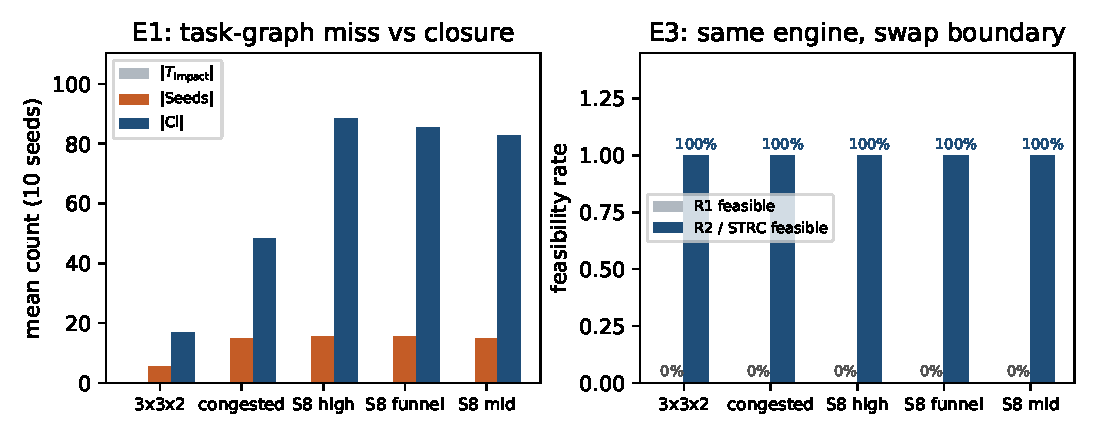
\includegraphics[width=\linewidth]{figures/fig_strc_e1e3}
\caption{E1/E3 扩样可视化(\(\NInst\) 算例 \(\times\) \(\NSeeds\) 种子均值)。
左:任务图影响域为空而种子与闭包非空;
右:同改路引擎下仅换边界时 R1 可行率为 \(0\)、R2 为 \(100\%\)。}
\Description{并排两幅条形图。左幅按五个算例给出任务图影响域、种子数与闭包规模
三组柱子,影响域一组恒为零,另两组随算例规模上升。右幅给出两条边界定义的恢复
可行率,任务图边界一侧为零,闭包一侧为百分之百。}
\label{fig:e1e3}
\end{figure}

%% 标题里不放 \(\times\):它会进 PDF 书签,hyperref 无法处理数学模式。
\subsection{E6:扰动类型与边界定义的交叉}
\label{sec:e6}

E1--E3 只用了走廊阻断一种扰动。本小节把扰动类型这一维展开,在同一 \(\NPairs\) 对上另加
路段降速、车辆故障与机械臂故障三类,填满表~\ref{tab:e6} 这张覆盖矩阵。

\textbf{先说这一组只测什么、不测什么。} 四类扰动中只有走廊阻断被修复引擎正确建模——
阻断以强制占用注入路由层(第~\ref{sec:level1}~节)。降速在当前实现中被当作整段阻断处理,
是一个过近似;车辆故障与机械臂故障则没有对应的注入通道,重放时那台车/那台机器仍然可用。
若对后三类照跑「可行率」,得到的会是假阳性。因此 E6 \emph{只报边界}:
任务图影响域有多大、预约闭包有多大、后者是否包含前者。
这恰好是覆盖矩阵要回答的问题——「任务图边界看不看得见这类扰动」——而它不需要修复语义。

\begin{table}[t]
\centering
\caption{E6 扰动类型 \(\times\) 边界定义(\(\NPairs\) 对/类,共 \(200\) 次测量)。
\(|R^{\circ}|\) 为 \(t_{\mathrm{now}}\) 之后的活预约数。
「R1 为空」即任务图边界判该扰动无需重调度的格数。}
\label{tab:e6}
\small
\begin{tabular}{@{}llcccc@{}}
\toprule
扰动 & 类 & R1 为空 & 均 \(|U_{R1}|\) & 均 \(|\mathrm{Cl}|\)
 & \(\mathrm{Cl}/|R^{\circ}|\) \\
\midrule
走廊阻断   & B & \(50/50\) & \(0.0\)  & \(62.6\) & \(0.90\) \\
路段降速   & B & \(50/50\) & \(0.0\)  & \(62.6\) & \(0.90\) \\
车辆故障   & A & \(0/50\)  & \(31.1\) & \(53.0\) & \(0.75\) \\
机械臂故障 & A & \(0/50\)  & \(42.8\) & \(62.7\) & \(0.90\) \\
\bottomrule
\end{tabular}
\end{table}

三点读数。第一,\textbf{A/B 二分在 \(200\) 次测量上无一例外}:两类 B 扰动的任务图边界
全部为空,两类 A 扰动全部非空。第二,\textbf{在全部 \(100\) 次 A 类测量上
\(U_{R1}\subseteq\mathrm{Cl}\)}——这说明改用闭包边界在 A 类上不会\emph{丢失}
任务图能看见的东西。包含在 \(\StrictlyLarger\) 上是严格的,其余 \(19\) 格两者恰好相等
(此时闭包沿依赖边没有走出任务图影响域诱导的那个集合),\emph{不是}包含失败。
代价是释放集平均变大:车辆故障 \(31.1\to 53.0\),机械臂故障 \(42.8\to 62.7\)。
结合第一点,闭包边界在这四类扰动上是任务图边界的一致加强,而非另一种取舍。
第三,\textbf{降速与阻断两行逐格相同},在全部 \(50\) 对上闭包规模一致。
这不是两次独立的验证:本文的种子规则对二者都是「与失效时窗重叠的活预约」,
故它们按构造给出同一个种子集,进而给出同一个闭包。该行证实的是任务图边界对降速同样为空,
不是对 B 类结论的重复确认。

\textbf{这张表也给出了不作最小性主张的实测依据}(注~\ref{rem:minimality})。
走廊阻断下闭包覆盖 \(t_{\mathrm{now}}\) 之后活预约的约 \(\ClosureAliveFrac\);
相对「释放全部未来」这一平凡上界只省下一成。有界修复真正省下的是不动过去与不重开搜索,
而不是把未来切得很小。第~\ref{sec:e1}~节按全表统计的 \(\mathrm{Cl}/|R|\approx 0.57\)
与此不矛盾:全表包含 \(t_{\mathrm{now}}\) 之前已经执行完毕、按假设 A1 本就不可改的那一半。
两个口径都给出,以免读者只看到有利的那个。

\subsection{案例甘特}
\label{sec:case}

\begin{sloppypar}
E1--E3 给出的是跨种子的计数与可行率。为把「任务图覆盖不到、闭包可修」落到时间轴上,
图~\ref{fig:case} 取 \texttt{example\_3x3x2}、种子 \(42\) 的一例走廊阻断,
协议同 E2/E3:决策时刻取 \(0.35\,C_{\max}\),繁忙走廊单窗阻断,第 1 级改路、无扩域。
\end{sloppypar}

该例上 \(T_{\mathrm{impact}}=\varnothing\),而 \(|\mathrm{Seeds}|=6\)、\(|\mathrm{Cl}|=16\)。
图~\ref{fig:case}(a) 为扰动前原排程的机器甘特:蓝色工序的运输预约落入闭包(将被释放改路),
灰色工序在闭包外(预提交冻结);红色虚线为 \(t_{\mathrm{now}}\),浅红带为阻断时窗。
图~\ref{fig:case}(b) 为修复后:闭包内工序时间轴重排,排程在阻断下恢复可行,
\(C_{\max}:57\to 86\),耗时亚毫秒级。
本图不用于宣称完工时间最优——它只说明统计结论对应何种局部改动形态;
完工时间与全局重解的权衡见随后的 E5 与规模扫描。

\begin{figure}[t]
\centering
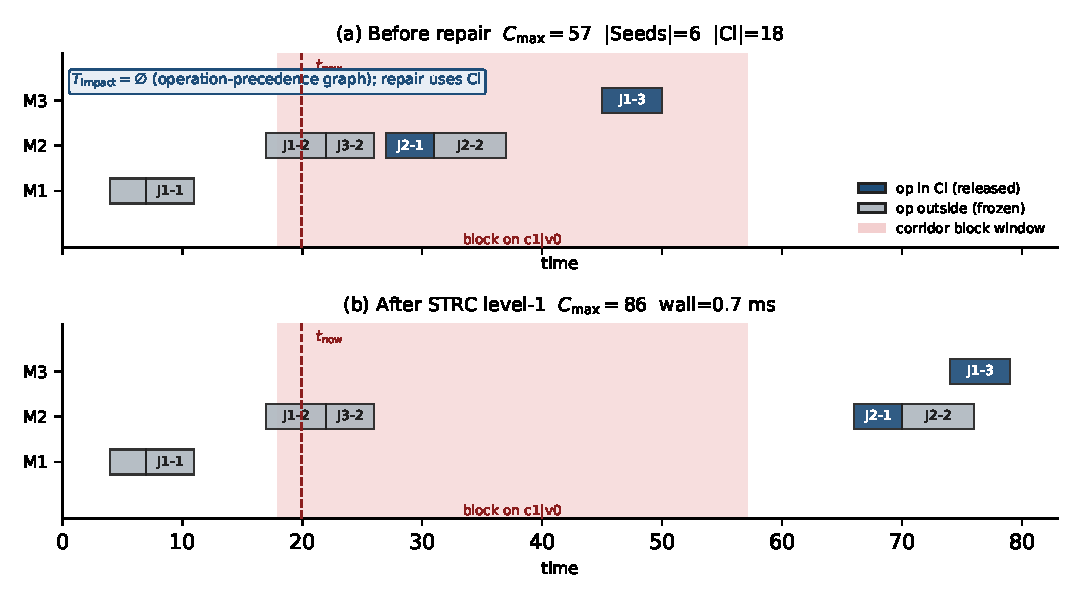
\includegraphics[width=\linewidth]{figures/fig_strc_case}
\caption{案例甘特(\texttt{example\_3x3x2}, seed \(42\))。
(a)~阻断前原排程,按是否属于 \(\mathrm{Cl}\) 着色;
(b)~STRC 第 1 级修复后。任务图影响域为空;蓝色工序对应闭包内运输被改路。}
\Description{上下两幅机器甘特图。(a) 阻断前的原排程,条块按其运输预约是否落在
闭包内着蓝灰两色,一条竖直红虚线标出决策时刻,一条浅红竖带标出阻断时窗。
(b) 修复后的排程,蓝色条块的时间轴被重排,灰色条块位置不变,完工时间由 57 增至 86。}
\label{fig:case}
\end{figure}

\subsection{E4:结构(探索)}
\label{sec:e4}

在 LU 割边阻断下,funnel 与 high 的闭包占比随种子波动(表~\ref{tab:e4})。
方向上确实是 funnel 更高——中位 \(0.254\) 对 \(0.204\),均值 \(0.244\) 对 \(0.229\)
——但\emph{两组取值高度重叠}:funnel 落在 \([0.180,0.309]\),high 落在
\([0.156,0.372]\),后者的区间把前者整个包住,且单个种子即可反向
(\(2024\) 一列上 high 的 \(0.372\) 反高于 funnel 的 \(0.296\))。
五个种子、两个布局,这个差距不足以支撑任何结论。
第~\ref{sec:e1}~节按繁忙走廊阻断协议在三个同规模布局上得到的
\(\mathrm{Cl}/|R|\) 亦落在 \(0.54\)--\(0.57\) 的窄带内,同样未能区分布局。

\textbf{换一批不由本文设计的布局,这条负结果的成因才分得清.}
上述三张同规模布局同属哑铃一族,彼此只差并行通道数,也就是只差容量、不差几何;于是
"指标太粗"与"算例集本身几何差异不足"这两种解释在它们身上是混在一起的,无从分辨。
第~\ref{sec:protocol}~节第二批把两者分开了(表~\ref{tab:e4pub})。

\textbf{结果的方向与预期相反,而这恰是关键.}
按第~\ref{sec:protocol}~节的声明,这批算例在路网几何上只有 \NPubNets\ 个独立样本,
故\emph{不能}用它来论证"闭包占比随路网几何变化";能论证的是另一件事,而且更有力。
在\emph{同一张} \(4\times 4\) 路网上,只把机器台数与落位从 \(4\) 机换成 \(5\) 机,
闭包占比中位即由 \PubCloHi\ 落到 \PubCloLo,极差 \PubCloSpread;
同一张 \(5\times 5\) 路网上换三种落位,极差 \PubCloSpreadBig。
作为对比,\emph{逐参数同口径}的三张自建布局——它们是三张\emph{不同}的路网——
只落在 \SelfCloLo--\SelfCloHi,极差 \SelfCloSpread。
即:\textbf{路网固定、只动机器落位,闭包占比的变动幅度可以超过换三张不同路网的幅度}
——\(4\times 4\) 那张上是约四倍,\(5\times 5\) 那张上约一点五倍。两张路网上都成立的是
不等号的方向,倍数本身只有两个样本,不宜细读。

\textbf{于是静态割被干净地否证了.}
在这 \NPubInst\ 个外部算例上,\textbf{LU 最小割恒为 \(2\)、漏斗占比恒为 \(0\)}——
两张路网都把装卸站放在网格角点,而四邻接网格的角点恰有两条出边,这个割因此被钉死。
同一工具集另附的那族布局(即因允许对角移动而未收入的一族)把装卸站放在网格边的中点,
其出边数是 \(3\)——换言之,\textbf{这个指标在真实布局上只取到极少数几个由"装卸站摆在
哪种网格位置"决定的值},并不随几何连续变化。
关键在于:\textbf{这两个指标在上述整段变动中一动不动},而被解释的量已经变了
\PubCloSpread。一个取值恒定的量不可能解释一个如此变动的量,所以它们连"相关性弱"都
谈不上,是\emph{无从谈起};第三个指标(每节点走廊数)虽有两个取值,与闭包占比的秩相关为
\(0\)。

据此可把原先那句含糊的观察收紧为一条明确的否证:\textbf{闭包规模不由装卸点处的静态割
决定}。最小割这一族指标本是围绕哑铃布局那个可调的 LU 咽喉设计出来的,迁到真实布局上就
退化成常量,不具备解释力。因此本文\textbf{不}把「闭包规模由争用结构决定」列为贡献。
更进一步,上面那组读数指出了替代方向:既然路网不变而落位一变,闭包占比就大幅移动,
那么决定闭包规模的不是路网\emph{能}提供多少条通路,而是\emph{需求落在哪里}——
应当刻画的是 \(t_{\mathrm{now}}\) 邻域内走廊占用的\emph{时序}密度,而不是静态拓扑的
连通度(第~\ref{sec:future}~节)。

\begin{table}[t]
\centering
\caption{E4 闭包占比 \(\mathrm{Cl}/|R|\)(LU 割边阻断;种子 \(42,7,2024,99,123\))。
本表算例为 \(12\) 工件 / \(8\) 机 / \(12\) 车、运输与加工时长比标定为 \(4.0\)。
\textbf{该口径与表~\ref{tab:e4pub} 不同}(后者为 \(8\) 工件 / \(4\) 机 / \(4\) 车、
比值 \(1.0\)、十种子),两表虽共用 \texttt{funnel}/\texttt{high} 这两个布局名,
\emph{数值不可跨表比较};表~\ref{tab:e4pub} 内部才是同口径对照。}
\label{tab:e4}
\small
\begin{tabular}{@{}lcccccc@{}}
\toprule
布局 & \(42\) & \(7\) & \(2024\) & \(99\) & \(123\) & 中位 \\
\midrule
funnel & \(0.254\) & \(0.181\) & \(0.296\) & \(0.309\) & \(0.180\) & \(0.254\) \\
high & \(0.156\) & \(0.204\) & \(0.372\) & \(0.229\) & \(0.184\) & \(0.204\) \\
\bottomrule
\end{tabular}
\end{table}

\begin{table}[t]
\centering
\caption{E4 布局出处外部化对照(LU 割边阻断,十种子;\(\mathrm{Cl}/|R|\) 取中位)。
全表逐参数同口径,只差路网与机器落位。\textbf{外部算例只落在 \NPubNets\ 张路网上}
(\(\mathrm{N}_1\):\(4\times 4\) 去一条边;\(\mathrm{N}_2\):\(5\times 5\) 去两条边),
组内各行\emph{共享同一路网},只差机器台数与落位;"极差"一列按\emph{组内}给出。
要点:\(\mathrm{N}_1\) 组内路网不变、仅换落位即得极差 \PubCloSpread,已是三张\emph{不同}
自建路网之间极差 \SelfCloSpread\ 的约四倍;而 LU 最小割与漏斗占比在整个外部批
\emph{取值恒定},故无从解释这些差异。
边权为本文补齐的等权值,故本表不与外部文献的参照值比较。}
\label{tab:e4pub}
\small
\begin{tabular}{@{}llcccccc@{}}
\toprule
出处/路网 & 算例 & 机器 & 节点/走廊 & LU 割 & 漏斗占比 & \(\mathrm{Cl}/|R|\)
 & 组内极差 \\
\midrule
外部 \(\mathrm{N}_1\) & \texttt{LyuL2} & \(4\) & \(16/23\) & \(2\) & \(0\) & \(0.512\) & \\
外部 \(\mathrm{N}_1\) & \texttt{LyuL3} & \(5\) & \(16/23\) & \(2\) & \(0\) & \(0.305\)
  & \(\PubCloSpread\) \\
\cmidrule{1-8}
外部 \(\mathrm{N}_2\) & \texttt{LyuL4} & \(6\) & \(25/38\) & \(2\) & \(0\) & \(0.385\) & \\
外部 \(\mathrm{N}_2\) & \texttt{LyuL5} & \(7\) & \(25/38\) & \(2\) & \(0\) & \(0.422\) & \\
外部 \(\mathrm{N}_2\) & \texttt{LyuL6} & \(8\) & \(25/38\) & \(2\) & \(0\) & \(0.460\)
  & \(\PubCloSpreadBig\) \\
\midrule
自建 & \texttt{high} & \(4\) & \(10/10\) & \(2\) & \(0.286\) & \(0.497\) & \\
自建 & \texttt{funnel} & \(4\) & \(9/8\) & \(1\) & \(0.286\) & \(0.491\) & \\
自建 & \texttt{mid} & \(4\) & \(11/12\) & \(2\) & \(0.286\) & \(0.446\)
  & \(\SelfCloSpread\) \\
\bottomrule
\end{tabular}
\end{table}

\subsection{E5:与全局重解的权衡}
\label{sec:e5}

本小节的设计意图原是找一个\emph{交叉点}:预算紧时有界修复占优,预算放宽后热启动全局重解
反超。\textbf{该交叉点不存在},本文如实报告这一结果,并据此改写机制层的定位。

表~\ref{tab:e5} 与图~\ref{fig:e5} 在两个算例上对种子 \(\{42,7,2024\}\) 扫描 R0+ 预算
\(\{0.2,1,2\}\)\,s,共 \(2\times3\times3=18\) 个预算点。R0+ 即使在\emph{最小}预算
\(0.2\)\,s 下也已优于 R2,且随预算继续拉开;在全部 \(18\) 个点上无一例外。

\begin{table}[t]
\centering
\caption{E5 与热启动全局重解的权衡(\(3\) 种子均值)。
「改动比例」为被改写的预约占全表之比。\(C_{\max}\) 一列 R0+ 全区间更优。}
\label{tab:e5}
\small
\begin{tabular}{@{}lcccc@{}}
\toprule
算例 & 预算/s & R0+ \(C_{\max}\) & R2 \(C_{\max}\) & 改动比例 R0+ / R2 \\
\midrule
\multirow{3}{*}{\texttt{congested\_8x4x4}}
 & \(0.2\) & \(221.3\) & \(299.0\) & \(0.99\) / \(0.57\) \\
 & \(1.0\) & \(198.3\) & \(299.0\) & \(1.00\) / \(0.57\) \\
 & \(2.0\) & \(142.7\) & \(299.0\) & \(1.00\) / \(0.57\) \\
\addlinespace[2pt]
\multirow{3}{*}{\texttt{example\_3x3x2}}
 & \(0.2\) & \(45.7\)  & \(88.7\)  & \(0.97\) / \(0.60\) \\
 & \(1.0\) & \(45.3\)  & \(88.7\)  & \(0.97\) / \(0.60\) \\
 & \(2.0\) & \(45.3\)  & \(88.7\)  & \(0.97\) / \(0.60\) \\
\bottomrule
\end{tabular}
\end{table}

\begin{figure}[t]
\centering
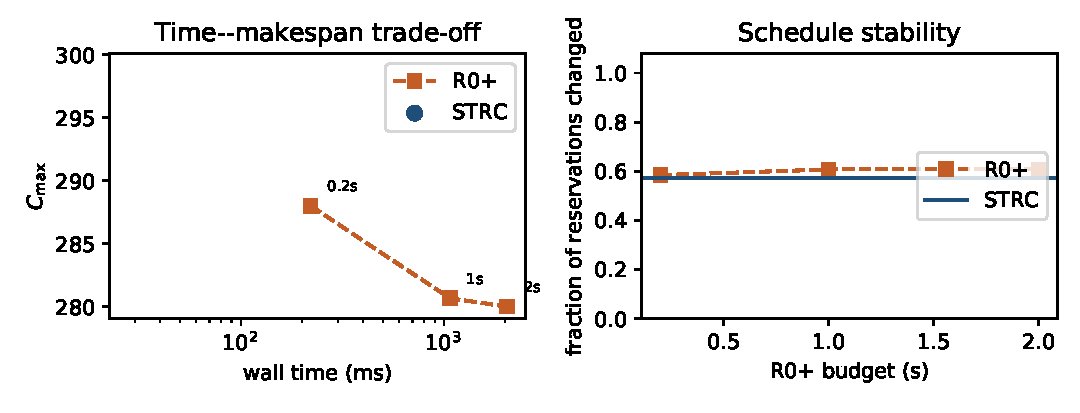
\includegraphics[width=\linewidth]{figures/fig_strc_e5}
\caption{E5:R0+ 预算扫描与 STRC 定点(\texttt{congested\_8x4x4}, \(3\) 种子均值)。
左:耗时--\(C_{\max}\),两条曲线不相交;右:预约改动比例。}
\Description{并排两幅图。左幅横轴为对数刻度的响应耗时、纵轴为完工时间:
热启动全局重解随预算增加沿曲线下行,有界修复是左上方的一个定点,
两者不相交,全局重解在每个预算点上都更低。右幅为预约改动比例的条形对比,
全局重解接近百分之百,有界修复约六成。}
\label{fig:e5}
\end{figure}

\textbf{据此改写角色分工的表述。} 有界修复在\emph{时间}(低两至三个数量级)与
\emph{稳定性}(改动 \ResFracRtwo{} 的预约,而 R0+ 改动 \ResFracRzero{})
两个维度上大幅占优,在\emph{解质量}上全区间劣势。诚实的定位是:

\begin{quote}
有界修复不是「更好的重调度」,而是「\emph{必须立刻给出可执行方案、且不愿撕毁已下发承诺}
时」的那一档。若允许秒级停机并接受近乎全盘改写,热启动全局重解在完工时间上占优。
\end{quote}

需要说明为什么不换指标绕过去。若改用「相对初始解的 \(C_{\max}\) 退化率」或
「\(C_{\max}\) 与改动比例的加权和」,R2 都会好看一些,但那是在事后挑一个对自己有利的
标量化方式。\(C_{\max}\) 是本领域的主指标,本文在它上面输了,就按它报。
这条读数也约束了前文的用词:第~\ref{sec:vs_r0}~节所说的「互补」,
指的是两者在\emph{响应时间}这一约束下各自占据的区间,不是指存在某个预算区间使 R2 更优。

\textbf{但有一处口径必须交代:该对照臂并未受假设 A2 约束。} 它是从 \(t=0\) 重新解码
整条排程的,因而可以重排 \(t_{\mathrm{now}}\) 之前\emph{已经执行完毕}的占用,而
假设 A2(第~\ref{sec:assumptions}~节)不允许恢复方案这样做。用注~\ref{rem:e2b_history}
所述的历史不可改写审计逐点检查:在本节的 \(18\) 个预算点上,该臂改写了
\(\RzeroPastLo\)--\(\RzeroPastHi\) 的已完成预约,\emph{无一点为零};作为对照,
有界修复在同样 \(6\) 个算例--种子格上一律为零(更宽的 \(\NPairs\) 对上亦然)。
假设 A5 确实为该臂开过一个口子——允许它改动染色体——但那是\emph{动作}维度上的豁免,
不含\emph{时间}维度。

因此上表 R0+ 一列宜读作\textbf{参考下界}:它回答的是「若允许回溯重排历史、且给足秒级
预算,完工时间能低到什么程度」,而不是一个可采纳恢复方案的成绩。
需要强调的是,\emph{这一澄清不改变本节的结论}:\(18/18\) 的读数与「不存在交叉点」的
表述照原样保留。原因是本文并\emph{未}给出一个受 A2 约束的全局重解对照,因而无从声称
在那样的对照下结果会不同——把这个对照臂补上是后续工作(第~\ref{sec:future}~节)。

\subsection{E7:便宜的可采纳对照}
\label{sec:cheap}

上一节的对照臂是热启动种群搜索,预算 \(0.2\)--\(2\)\,s。只用它作对照会留下一个显然的
反问:\emph{「低两至三个数量级」这个读数,有多少来自闭包本身,又有多少只是因为对照选贵了?}
本节把阶梯中间那两档便宜的全局重算补上。

\begin{itemize}[leftmargin=1.5em,itemsep=0.25em]
\item \textbf{RS(全局右移)。} 不改路径、不改指派、不改扫描序,把未完成的一切统一后推
一个延迟 \(\Delta\),\(\Delta\) 取到刚好让受阻走廊上所有可动的占用落到阻断窗之后。
冻结判据与 R2 相同(\(t_{\mathrm{end}}\le t_{\mathrm{now}}\) 不可动),故它按假设 A2
是可采纳的;因为是统一平移,一切间隔要么不变、要么变大,而全部约束都是「\(\ge\)」型,
无需重新路由即得可行解。它是「\emph{不划边界}」的一端:连重路由都放弃
(第~\ref{sec:rw_aor}~节)。
\item \textbf{RD(原染色体重解码)。} 保持机器指派与扫描序,在装了阻断的路由层上从头
解码一遍。它是本文实现里\emph{最便宜的一次全局重算}——种群搜索每评估一个候选都至少要付
这笔钱。但它从 \(t=0\) 重排,\textbf{不受 A2 约束},故其 \(C_{\max}\) 须连同越界格数一起读。
\item \textbf{RA(不划边界,但保留重路由)。} 释放 \(t_{\mathrm{now}}\) 之后的\emph{全部}预约,
再走与 R2 \emph{完全相同}的改路重放。它是「不划边界」的另一端:与 RS 不同,它保留了
重路由这一动作,因而与 R2 只差释放集这一项。它与 R2 共用修复引擎、共用冻结判据、共用阻断安装,唯一
差别是释放集取了平凡上界而非闭包。因此它是本文\emph{唯一}能把闭包这个对象单独隔离
出来的对照:两臂之差不含引擎、协议或实现的贡献。它同样按 A2 可采纳,且已是最大释放集,
无需失败扩域。
\end{itemize}

设置 RA 的必要性来自一个尖锐的反问。闭包既然已经覆盖了活预约的约
\ClosureAliveFrac(注~\ref{rem:minimality}),那么\emph{划这条边界还剩多少用}?
E3 比较的是两种\emph{不同}的边界定义(任务图 vs 时空闭包),而 RA 问的是更根本的
一层:\emph{要不要边界}。

\begin{table}[t]
\centering
\caption{E7 便宜对照臂(\(\NPairs\) 对,协议与 E3 相同:繁忙走廊单窗阻断、
\(t_{\mathrm{now}}=0.35\,C_{\max}^{0}\)、R2 不开失败扩域)。四臂均 \(\NPairs/\NPairs\) 可行。
「A2 越界」为改写了已完成预约的格数;「释放集」为该臂释放的预约占 \(t_{\mathrm{now}}\)
之后活预约的比例;末列为该臂对 R2 的 \(C_{\max}\) 胜负。RA 与 R2 只差释放集,
故这两行之差可全部归因于闭包本身。本表\emph{不可}与表~\ref{tab:e5} 并读——那批只有两个算例。}
\label{tab:cheap}
\small
\begin{tabular}{@{}lcccccc@{}}
\toprule
臂 & A2 越界 & ms(中位) & 平均退化 & 改动比例 & 释放集 & 对 R2 赢/平/输 \\
\midrule
RS 全局右移      & \ShiftBad     & \MsShift    & \(58.8\%\) & \ResFracShift    & ---   & \(7/16/27\) \\
RD 重解码        & \RedecodeBad  & \MsRedecode & \(46.5\%\) & \ResFracRedecode & ---   & \(25/23/2\) \\
RA 不划边界      & \ShiftBad     & \MsAllFuture & \(49.9\%\) & \ResFracAllFuture & \(1.00\) & \(0/46/4\) \\
R2 闭包有界修复  & \ShiftBad     & \MsCheapRtwo & \(49.8\%\) & \ResFracCheapRtwo & \ClosureShareMean & --- \\
\bottomrule
\end{tabular}
\end{table}

表~\ref{tab:cheap} 给出四条读数。

\textbf{其一,在给出可行方案的各臂中,唯一比有界修复更快的是全局右移,
而它在解质量与稳定性上都输。}(任务图边界臂 R1 更快,但它在 \FeasRone\ 上恢复可行,
不构成候选。)
RS 只要 \MsShift\,ms,约为 R2 的一半;代价是完工时间平均退化 \(58.8\%\)(R2 为
\(49.8\%\)),逐格对比 \WinVsShift(R2 赢/平/输),且改动的预约反而更多
(\ResFracShift\ 对 \ResFracCheapRtwo)——统一平移把每一条未来预约的时刻都改了。
值得指出的是,若想把右移做得\emph{有选择}——只推迟真正受影响的车,其余不动——就必须先
知道哪些预约受影响,那正是本文定义的那个边界。\textbf{右移之所以能不划边界,恰恰因为
它放弃了选择。}

\textbf{其二,最便宜的一次全局重算比一次有界修复更贵。} RD 的耗时中位是
\MsRedecode\,ms,为 R2 的 \(2.3\) 倍。这条读数与搜索配置无关:任何基于解码的搜索,
每评估一个候选都要付至少一次解码的代价。因此上一节「低两至三个数量级」并\emph{不}是
选贵了对照造成的——把对照换成同一实现里最便宜的那一档,有界修复仍然更快。

\textbf{其三,RD 在完工时间上更好,但那部分优势主要来自越界。} 全表看 R2 对它是
\WinVsRedecode(赢/平/输),而它在 \RedecodeBad\ 个格上改写了已经执行完毕的占用——与
第~\ref{sec:e5}~节对全局重解臂的口径说明是同一回事,只是程度轻些。按越界与否分层后
差距明显收窄:在 RD \emph{恰好}没有越界的 \(19\) 个格上,R2 赢 \(1\)、平 \(9\)、输 \(9\),
两臂基本持平(第~\ref{sec:instscale}~节的 \(46\) 个同类格上为赢 \(5\)、平 \(22\)、输 \(19\))。
须强调「恰好」二字:RD 并非受 A2 约束的算法,它只是在这些格上没有用到那份自由度,
因此这一分层给出的是差距的\emph{上界估计},不是一个受约束对照的成绩——那仍是
第~\ref{sec:future}~节的第一件事。

\textbf{其四,闭包换来的是稳定性,而且只换来稳定性。} RA 与 R2 只差释放集,因此这一对
读数直接回答了「划这条边界值不值」。闭包平均只比平凡上界少放 \(1-\ClosureShareMean\)
的活预约(逐格 \ClosureShareLo--\(1.00\),取到 \(1.00\) 的 \(4\) 个格上闭包\emph{就是}
全部未来预约,两臂恒等)。就是这不足一成的差别,换来了改动比例从 \ResFracAllFuture\ 降到
\ResFracCheapRtwo:平均降 \RAStabMean、中位降 \RAStabMed,逐格 \RAStabWTL(R2 更稳/持平/更差),
Wilcoxon 符号秩双侧 \(p=\RAStabP\)。方向高度一致,\emph{幅度不大}——唯一的反例格降幅为
\(+0.007\),可忽略但如实记录。与此同时耗时几乎相同(\MsCheapRtwo\ 对 \MsAllFuture\,ms),
完工时间也几乎相同(比值均值 \RACmaxRatio,逐格 R2 赢/平/输 \WinVsAllFuture、从未更差,
最占优的一格为 \RACmaxLo)。

这三项各自都该如此,合起来才是重点。\textbf{耗时相同,说明「毫秒级响应」这个读数不来自
闭包,而来自「单遍改路、不重开搜索」——这一点本文本就不主张新颖(表~\ref{tab:position})。
完工时间相同,说明闭包不是一种优化手段。改动比例显著更低,说明闭包兑现的恰是命题
\ref{prop:outside} 承诺的那个量:外侧字段不变。}换言之,闭包的价值不在快、也不在好,
而在\emph{知道哪些不必动}——这正是一个「边界」应该提供的东西,也解释了为什么幅度与闭包
排除掉多少成正比:在闭包接近全部未来预约的算例上(\texttt{congested\_8x4x4},释放占比
\(0.94\))降幅只有 \(0.010\),而在闭包排除得多的算例上(\texttt{S8x4x4\_mid},\(0.88\))
降幅达 \(0.128\)。

四臂并读的结论是:在「按 A2 可采纳、且响应在毫秒量级」这两个约束下,
\textbf{唯一比有界修复更快的做法(全局右移)在解质量与稳定性上都更差;唯一在解质量上
更好的做法(重解码)既更慢、又在多数格上不可采纳;而在同等速度与同等解质量下,
不划边界要多改约 \(7\) 个百分点的预约(相对多约一成三)}。
放宽前两个约束,更好的完工时间都能买到,但买到的不再是一个可采纳的恢复方案。

\subsection{扰动规模扫描}
\label{sec:scale}

表~\ref{tab:scale} 与图~\ref{fig:scale} 报告 \(\varphi\) 扫描
(\texttt{congested\_8x4x4}, \(\NSeeds\) 种子; R0+ 预算 \(2\)\,s; STRC 含失败扩域)。
两臂可行率均为 \(100\%\); STRC 耗时约 \(8\)--\(11\)\,ms,R0+ 约 \(2\)\,s;
\(C_{\max}\) 仍全由 R0+ 更优,与第~\ref{sec:e5}~节一致。
小例 \texttt{example\_3x3x2} 上同样每格可行(\(\NSeeds\) 种子 \(\times\) 五个
\(\varphi\) 值),STRC 约 \(1\)\,ms 量级,
加速比 \(\SpeedLo\times\)--\(\SpeedHi\times\)(跨两个算例的逐格极值)。

这里 STRC 打开了失败扩域,故与 E3/E5 不可直接比较:扩域是把可行率\emph{兜}到 \(100\%\) 的
机制,而它本身并非本文首创(第~\ref{sec:rw_aor}~节)。本表的用途是说明,
即使在扰动比例升至 \(\varphi=1\)(全部未来工序受扰)时,闭包路径仍停留在十余毫秒量级,
响应时间不随扰动规模崩溃。

\begin{table}[t]
\centering
\caption{扰动规模对照(\texttt{congested\_8x4x4}, \(\NSeeds\) 种子平均)。
STRC 含扩域;R0+ 预算 \(2\)\,s。}
\label{tab:scale}
\small
\begin{tabular}{@{}rcccc@{}}
\toprule
\(\varphi\) & STRC 可行 & STRC\,ms & R0+ \(C_{\max}\) & 耗时比 \\
\midrule
\(0.10\) & \(100\%\) & \(9.1\)  & \(103.5\) & \(406\times\) \\
\(0.25\) & \(100\%\) & \(11.1\) & \(107.0\) & \(325\times\) \\
\(0.50\) & \(100\%\) & \(8.6\)  & \(111.8\) & \(333\times\) \\
\(0.75\) & \(100\%\) & \(8.4\)  & \(125.8\) & \(254\times\) \\
\(1.00\) & \(100\%\) & \(10.7\) & \(148.1\) & \(203\times\) \\
\bottomrule
\end{tabular}
\end{table}

\begin{figure}[t]
\centering
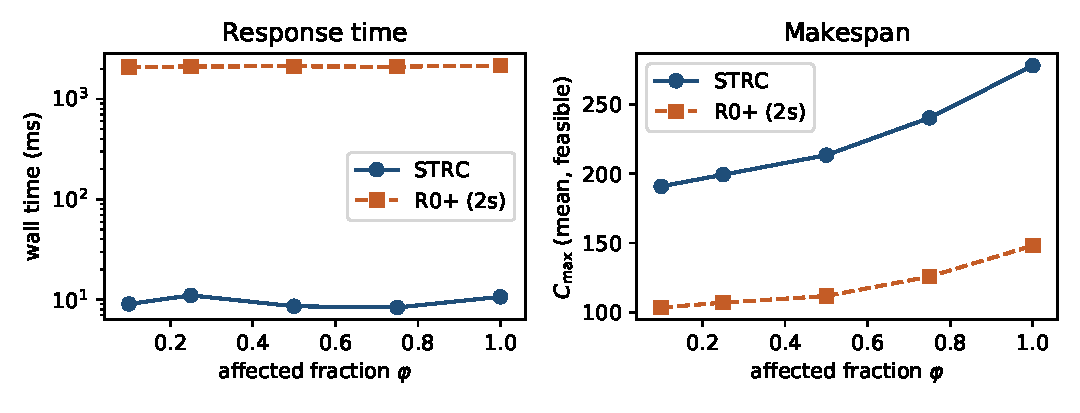
\includegraphics[width=\linewidth]{figures/fig_strc_scale}
\caption{扰动规模扫描(\texttt{congested\_8x4x4}, \(\NSeeds\) 种子):
响应时间(对数轴)与完工时间随 \(\varphi\) 变化。}
\Description{两条随扰动比例变化的曲线。响应时间画在对数纵轴上:有界修复始终在
十毫秒量级、不随比例上升而崩溃,全局重解固定在两秒的预算线上。完工时间一侧,
全局重解随扰动比例增大而缓慢上升,但始终低于有界修复。}
\label{fig:scale}
\end{figure}

\subsection{E8:算例规模上的外推}
\label{sec:instscale}

上一节扫的是\emph{扰动}的规模,算例始终是 \(8\) 工件 \(4\) 机。本节换一维:固定扰动协议,
把算例本身放大。这一问的要害不在耗时——耗时不崩是可以预期的——而在\textbf{闭包占比会不会
随规模涨到接近 \(1\),使「有界」名存实亡}。

梯子取工件数 \(2k\)、机器数 \(k\)、车数 \(k\),\(k=4,\dots,10\),即 \(8\times4\times4\) 到
\(\ScaleJobsHi\times\ScaleMachHi\times\ScaleMachHi\),共 \(\ScaleKs\) 档 \(\times\)
\(\NSeeds\) 种子 \(=\ScalePairs\) 对。拥堵档、异构度、柔性度、运输/加工时长比与装卸点
最小割、远端割全部按同一目标标定,\emph{只有规模变}。三条臂与第~\ref{sec:cheap}~节同定义。

\begin{table}[t]
\centering
\caption{E8 算例规模扫描(\(\ScaleKs\) 档 \(\times\) \(\NSeeds\) 种子)。
「闭包」为闭包预约占全表之比;耗时取中位。末列为 R2 对 RS 的 \(C_{\max}\) 胜负。}
\label{tab:instscale}
\small
\begin{tabular}{@{}lrccccc@{}}
\toprule
规模 & \(|R|\) & 闭包 & R2\,ms & RD\,ms & RD/R2 & R2 对 RS \\
\midrule
\(8\times4\times4\)    & \(148\) & \(0.544\) & \(3.8\)  & \(8.8\)  & \(2.3\times\) & \(7/1/2\) \\
\(10\times5\times5\)   & \(172\) & \(0.449\) & \(4.3\)  & \(12.8\) & \(3.0\times\) & \(9/0/1\) \\
\(12\times6\times6\)   & \(230\) & \(0.470\) & \(6.0\)  & \(20.4\) & \(3.4\times\) & \(7/1/2\) \\
\(14\times7\times7\)   & \(281\) & \(0.469\) & \(8.4\)  & \(28.5\) & \(3.4\times\) & \(8/0/2\) \\
\(16\times8\times8\)   & \(291\) & \(0.495\) & \(8.3\)  & \(32.1\) & \(3.9\times\) & \(10/0/0\) \\
\(18\times9\times9\)   & \(356\) & \(0.489\) & \(9.9\)  & \(50.2\) & \(5.1\times\) & \(10/0/0\) \\
\(20\times10\times10\) & \(402\) & \(0.426\) & \(11.8\) & \(65.4\) & \(5.5\times\) & \(10/0/0\) \\
\bottomrule
\end{tabular}
\end{table}

\textbf{闭包占比不随规模增长。} 从 \ScaleCloHi\ 降到 \ScaleCloLo,趋势甚至是缓降的。
这是本节最要紧的一条:有界性并未随规模被稀释。但须说明这不是一个渐近主张——
七档不足以拟合任何增长率,能说的只是在这段区间内它没有退化。

\textbf{响应时间随预约总数近似线性。} \(|R|\) 增至 \(2.7\) 倍时,R2 的耗时中位从
\(3.8\) 增至 \ScaleMsHi\,ms,仍在十毫秒量级。第 1 级改路的可行格数为 \ScaleFeasFirst;
唯一失败的一格(\(10\times5\times5\),种子 \(42\))由失败扩域在第 \(3\) 轮兜住,
总耗时 \(20.1\)\,ms、完工时间与首级尝试相同,故终可行为 \ScaleFeasAll。

\textbf{两个对照的差距随规模拉大,方向都对本文有利。} 最便宜的全局重算与有界修复的耗时比
从 \ScaleRatioLo\(\times\) 单调升到 \ScaleRatioHi\(\times\)——规模越大,重算一遍越不划算;
而对不划边界的右移臂,R2 的 \(C_{\max}\) 胜负从 \(7/1/2\) 变为最后三档的 \(10/0/0\)——
规模越大,「只动该动的」相对「整体后推」的优势越明显。

\textbf{口径限制。} 这条梯子只有一个拥堵档、一个算例随机种子(每档的算例本身由种子
\(42\) 生成),因而它检验的是\emph{规模}这一维,不能替代第~\ref{sec:protocol}~节主批次在
拥堵结构上的对照。第~\ref{sec:e6}~节的四类扰动交叉与第~\ref{sec:scale}~节的扰动规模扫描
也没有在这批算例上重跑。

\subsection{外部布局批次的复现}
\label{sec:pubrepro}

第~\ref{sec:protocol}~节第二批把布局出处换成外部来源后,\(\NPubPairs\) 个算例--种子对上
E1/E2/E3/E5 的读数与主批次\emph{逐项同向}(E4 是唯一被改写的一格,见本节末;
E5 与主批次的唯一差别是多出一个两臂持平的预算点,见下):
任务图漏报 \PubPassMiss(结构泄漏计 \(0\)),结构包含性 \PubPassClosed,
外侧字段逐条不变 \PubPassInvar;边界消融下第 1 级改路的可行格数为 \PubFeasRone,
闭包边界为 \PubFeasRtwo。E1 协议下的闭包占比逐布局中位落在
\PubEoneFracLo--\PubEoneFracHi,与主批次逐算例的 \(0.54\)--\(0.58\) 同量级。
与全局重解的权衡亦无变化:\PubEfiveNoCross\ 个预算点上 R0+ 的 \(C_{\max}\) 更优,
余下 \(1\) 点两臂持平(\texttt{LyuL6\_8m},种子 \(2024\),预算 \(0.2\)\,s),
没有一个点上有界修复更优,交叉点仍不存在,而有界修复的响应时间仍在毫秒量级、
R0+ 仍在秒量级。

这一批的意义\emph{不}在于给出新的性能数字,而在于把"这些现象是否只在本文自己设计的
布局上成立"这一问的答案钉住:B 类扰动使任务图边界失效、预约闭包包含之、闭包外字段
不受扰动,这三件事在一批不由本文选定的拓扑上同样成立。唯一被这批算例改写的结论是
结构可预测性(第~\ref{sec:e4}~节),而它本来就是负结果。

\subsection{小结}
\label{sec:exp_summary}

\begin{itemize}[leftmargin=1.5em,itemsep=0.25em]
\item 问题层(E1)与边界消融(E3)在 \(\NPairs\) 个算例--种子对上无一例外成立;
案例甘特把同一协议落到工序时间轴。
\item 覆盖矩阵(E6)在四类扰动 \(\times\) \(\NPairs\) 对上给出完整读数:
A/B 二分无例外,且 A 类上闭包边界一致包含任务图边界。
\item 结构包含性(E2a)与外侧字段\emph{逐条}不变(E2b)均满通过;但这只说明
命题~\ref{prop:outside} 的四条前提在本文协议下成立,命题仍只作充分条件
(注~\ref{rem:e2b_history} 记录了前提 (iii) 曾如何在实现上被悄悄破坏)。
\item 与全局重解的关系是\emph{在响应时间约束下}的分工,不是质量上的互有胜负:
毫秒 vs 秒、改动 \ResFracRtwo{} vs \ResFracRzero{},但 \(C_{\max}\) 全区间劣势、无交叉。
\item 便宜对照臂(E7)排除了「对照选贵了」这一疑问:在给出可行方案的各臂中,唯一比有界
修复更快的是不划边界的全局右移,而它在 \(C_{\max}\)(逐格 \WinVsShift)与稳定性
(\ResFracShift\ 对 \ResFracCheapRtwo)上都输;而同一实现里最便宜的一次全局重算(原染色体重解码)比一次
有界修复还贵 \(2.3\) 倍,且 \RedecodeBad\ 个格上改写了历史。
\item 同一批还把闭包单独隔离出来测了一次:换用「不划边界、释放全部未来」的对照臂(RA,
与 R2 共用引擎与冻结判据),耗时与 \(C_{\max}\) 几乎不变(逐格 R2 赢/平/输 \WinVsAllFuture),
改动比例却由 \ResFracCheapRtwo\ 恶化到 \ResFracAllFuture——逐格 \RAStabWTL,
\(p=\RAStabP\)。故毫秒级响应来自「单遍改路」而非闭包,\textbf{闭包兑现的是稳定性},
且降幅与它排除掉多少成正比。
\item 算例规模扫描(E8)把梯子推到 \(\ScaleJobsHi\) 工件 \(\ScaleMachHi\) 机:闭包占比
从 \ScaleCloHi\ 缓降到 \ScaleCloLo(有界性未随规模稀释),响应时间随预约总数近似线性
升至 \ScaleMsHi\,ms,而与两个对照的差距同向拉大。这是一段区间内的读数,不是渐近主张。
\item 闭包覆盖约 \(\ClosureAliveFrac\) 的活预约,本文不作最小性主张。
\item 结构可预测性(E4)是负结果,且换用外部来源布局后结论更硬:在\emph{同一张} \(4\times 4\)
外部路网上只改机器落位,闭包占比即变动 \PubCloSpread(已是三张\emph{不同}自建路网之间极差
\SelfCloSpread\ 的约四倍),而 LU 最小割与漏斗占比在整批外部算例上\emph{取值恒定},
无从解释这一变动。故闭包规模不作可预测性主张,并据此把替代方向指向需求侧的时序密度。
\item 两批算例承担不同的问题:主批次给出现象与机制,第二批只检验这些现象是否依赖本文
自选的布局。把布局出处换成外部来源后(\(\NPubPairs\) 对),E1/E2/E3/E5 的读数逐项复现,
无一条结论因换布局而改变(第~\ref{sec:pubrepro}~节)。第二批在全文中只用于收窄主张、
未曾用于支持任何一条,且只有 E4 一格必须两批合读(第~\ref{sec:protocol}~节)。
\end{itemize}


%% =====================================================================
\section{结论}
\label{sec:conclusion}
%% =====================================================================

\subsection{结论}

本文指认了一类任务图覆盖不到的级联损坏,并将影响边界重新定义在时空预约闭包(\STRC)上。
在 \(\NInst\) 算例 \(\times\) \(\NSeeds\) 种子共 \(\NPairs\) 对上:
走廊阻断的任务图影响域 \(\PassMiss\) 为空而原排程确已不可行;
同一修复引擎下仅替换边界定义时,任务图边界 \(\FeasRone\) 恢复可行而闭包 \(\FeasRtwo\);
闭包的结构闭合性 \(\PassClosed\) 成立,闭包外侧预约字段的逐条不变 \(\PassInvar\) 成立;
四类扰动 \(\times\) 两种边界的覆盖矩阵上 A/B 二分无例外,且 A 类上闭包边界一致包含
任务图边界。

主张的边界也已划清。让行关系这一建模对象、「局部重规划 + 外侧冻结」这一机制形态、
以及「失败后扩大释放域」这一策略,分别在铁路 alternative graph、多智能体路径规划与
Local Rescheduling 中早已存在,本文不作创新声称(第~\ref{sec:rw_claim}~节)。
本文主张的是三件事:该边界在\emph{两图分立}的模型层级上被划错了;
改画之后它是一个由图结构唯一确定、有闭合性、可测量的\emph{对象}而非启发式半径;
以及这个对象是一次\emph{测量}而不是一个\emph{决策}。

该对象买到什么,也已单独测过。把释放集从闭包换成「\(t_{\mathrm{now}}\) 之后的全部预约」
而保持引擎、冻结判据与协议不变时,耗时与完工时间几乎不动,改动比例却由
\ResFracCheapRtwo\ 恶化到 \ResFracAllFuture(逐格 \RAStabWTL,\(p=\RAStabP\);
第~\ref{sec:cheap}~节)。故毫秒级响应应归因于单遍改路这一机制形态——本文对它不作创新
声称——而\textbf{闭包兑现的恰是命题~\ref{prop:outside} 承诺的那个量:外侧不动}。
这也界定了收益的形状:它与闭包排除掉多少成正比,因而在闭包接近平凡上界时趋于消失。

\subsection{局限}
\label{sec:limitations}

以下四条按对结论的威胁程度排序,第~\ref{sec:future}~节逐条给出推进方向。

\begin{enumerate}[leftmargin=1.6em,itemsep=0.35em]
\item \textbf{完工时间上全区间劣于热启动全局重解,且不存在交叉点。}
在 \(18\) 个预算点上无一例外。本文买到的是响应时间与稳定性,卖掉的是解质量;
定位已按此改写(第~\ref{sec:e5}~节),但这仍是一条实质限制。
需一并说明该对照的口径:这个对照臂\emph{未}受假设 A2 约束,实测在这 \(18\) 个点上
改写了 \(\RzeroPastLo\)--\(\RzeroPastHi\) 的已完成预约,故其完工时间宜读作参考下界
而非可采纳方案的成绩。这不使本条限制失效——本文没有构造受 A2 约束的全局重解对照,
也就无从判断在那样的对照下差距会缩到多少,甚至是否仍然存在。补上该对照臂是
第~\ref{sec:future}~节的第一件事。
第~\ref{sec:cheap}~节已排除该结论的一种廉价解释(对照选贵了):换成同一实现里最便宜的
一次全局重算,有界修复反而更快,而完工时间上的劣势在按 A2 越界与否分层后收窄到基本持平。
但那一档同样不是受约束对照,分层只给出差距的上界估计。

\item \textbf{对闭包这个对象,本文知道的仍不够:保证不充要、边集未经独立检验、
释放集不紧、规模也不可由静态结构预测。} 四者分述。

\emph{(i) 命题~\ref{prop:outside} 只是充分条件},\(\PassInvar\) 不等于充要:
实验说明的是四条前提在本文协议下成立,不是它们可以省略。前提 (iii) 尤其脆弱——
只要实现以比预约更粗的粒度决定重规划范围,\(U\) 外的占用就会被顺带改写
(注~\ref{rem:e2b_history});本文没有给出一个能自动检出该类粒度错配的手段。
更需注意的是,逐条比对外侧字段(E2b)\emph{不足以}兜住这类错配:同一注记的后半段记录了
一次只发生在闭包\emph{内部}、因而 E2b 完全看不见的历史改写,它要靠一项独立的
历史不可改写审计才暴露出来。因此本文对该类缺陷的检出依赖于「事后想到该查什么」,
而非一个完备的检查。

\emph{(ii) 依赖边集是否穷尽物理耦合,并未验证}:E2b 满通过检验的是修复实现与释放集
定义是否一致,而\emph{不是}\(G_R\) 的四类边是否覆盖了世界上一切可能的传播通道——
后者需要一个独立于 \(G_R\) 的耦合真值,本文没有。注~\ref{rem:minimality} 的过近似讨论
只说明边集可能\emph{偏多},反方向仍未检验。

\emph{(iii) 不作最小性主张,且闭包确实不小}:它覆盖 \(t_{\mathrm{now}}\) 之后活预约的约
\(\ClosureAliveFrac\)(注~\ref{rem:minimality});相对「释放全部未来」这一平凡上界,
结构化释放省下的不足一成。这一条的\emph{代价}已实测(第~\ref{sec:cheap}~节的 RA 臂):
那不足一成的差别换来改动比例降 \RAStabMean(逐格 \RAStabWTL,\(p=\RAStabP\)),
而耗时与 \(C_{\max}\) 不变。所以限制不在于「闭包无用」,而在于\textbf{收益幅度不大且与
闭包排除掉多少成正比}——在闭包接近全部未来预约的算例上降幅仅 \(0.010\)。
换言之,闭包越接近平凡上界,划这条边界的意义越小,而本文没有给出\emph{何时}会如此的判据。

\emph{(iv) 闭包规模的结构可预测性未能建立,且已知不由装卸点处的静态割给出}:
最小割与漏斗占比都没有做出可复现的区分;换用外部来源布局后这一点变得更确定——这两个指标
在整批外部算例上\emph{取值恒定}(两张路网都把装卸站放在网格角点,四邻接下角点恰有两条
出边),而闭包占比在\emph{同一张}路网上仅换机器落位就变动 \PubCloSpread(第~\ref{sec:e4}~节)。
须注意这条否证的适用范围:外部算例在路网几何这一维只有 \NPubNets\ 个独立样本,故本文
否证的是「静态割能解释闭包规模」,\emph{不是}「路网几何与闭包规模无关」——后者需要更多张
互不相同的公开路网才能检验,而可得的公开路网就这么多。下一个候选刻画应是
\(t_{\mathrm{now}}\) 邻域内走廊占用的时序密度,本文未做。

\item \textbf{实现覆盖窄于框架所述:一类扰动、一档恢复动作、一次响应。}
\emph{扰动一维},只有走廊阻断被修复引擎正确建模:E6 的另外三类只报边界、不报可行率——
降速被当作整段阻断(过近似),两类故障没有注入通道(第~\ref{sec:e6}~节);因此覆盖矩阵
在「边界」一维是满的,在「修复」一维仍只有一格。
\emph{动作一维},受限于假设 A5:保持原机器指派与扫描序,只允许改路与扩域;换车、改派、
改序属于升级阶梯的后续级,本文未评估,而放开它们即向全局重解退化,「有界」也随之失去边界。
\emph{时间一维},由假设 A2、A3,扰动在 \(t_{\mathrm{now}}\) 完全已知且不叠加;
扰动流、预测误差与滚动响应均未涉及。
\emph{规模一维}的情况好一些但仍有限:第~\ref{sec:instscale}~节把梯子推到
\(\ScaleJobsHi\) 工件 \(\ScaleMachHi\) 机、\(\ScalePairs\) 对,闭包占比未随规模上升;
但那条梯子只有一个拥堵档与一个算例种子,\(\ScaleKs\) 档也不足以支撑任何渐近论断,
更大规模与更多结构下的行为仍未知。

\item \textbf{外部参照缺位:这一支没有可换的公开基准,算例出处只外部化了一半,
结论亦未在第二套实现上复现。}
带无冲突运输的柔性作业车间已有若干公开算例族,但\emph{执行期扰动}这一支没有:
公开族发布的都是静态问题的输入。更硬的一层障碍在算例格式——主流族把运输时间发布为机器间
\textbf{行程时间矩阵}而不是路网,我们对两族共 \(11\) 张布局逐张检验过
\cite{homayouni2021production,bilge1995time},\emph{没有一张}能还原成与所发布矩阵一致的
无向走廊图(全部不对称,即同一对位置往返时长不等;其中两张连有向图也还原不出,因为违反
三角不等式)。矩阵里没有走廊,就没有走廊占用,于是 \(R\)、\(G_R\)、\(\mathrm{Cl}(\cdot)\)
与 B 类扰动在这类算例上\emph{一概无从定义}。这比静态工作受到的约束更紧:静态工作可以把
争用约束退化掉,退化后求解的仍是文献求解的那个问题,因而仍能借公开算例标定搜索能力;本文
没有这条退路——退化掉争用,被研究的对象本身就不存在了。
唯一发布显式双向排他路网的是 Lyu 等~\cite{lyu2019approach}。本文已按其附录布局做出第二批
算例(第~\ref{sec:protocol}~节),\textbf{布局因此不再由本文设计};但外部化只做到拓扑一层
——\emph{逐段行驶时间与工件数据仍是本文的}。前者原文未随该批布局发表(只随单个示例算例
给出,且取值并不均匀),后者若一并借用,公开族过低的运输/加工时长比会使争用现象直接消失。
所以这批算例\textbf{不能}用来复现 Lyu 或 van Os~\cite{vanos2026exact} 的参照值;后者的模型
另有「一个节点同时只容一车」的约束,与本文的走廊排他语义也不是同一回事。算例出处这一条
因此只解决了一半:布局那一半解决了,时间标定那一半没有。
外部批次的\textbf{覆盖范围也窄于主批次}:它复现的是 E1/E2/E3/E5(第~\ref{sec:pubrepro}~节),
E6 的四类扰动交叉、扰动规模扫描以及第~\ref{sec:cheap}~与~\ref{sec:instscale}~节的两批
(便宜对照臂、算例规模)都没有在外部布局上重跑;这四项的读数目前只有自建算例支撑。
此外,该批的 \NPubInst\ 个算例只落在 \NPubNets\ 张路网上(第~\ref{sec:protocol}~节),
路网几何这一维的样本量因此很小。
最后,下层路网、时间窗路由与校验器\textbf{与静态一体化工作复用同一实现}:这保证了归因的
干净,但也意味着上述结论尚未在第二套独立实现上复现。
\end{enumerate}

\subsection{后续工作}
\label{sec:future}

下列四件与上一节的四条局限一一对应。

\textbf{一、构造一个受假设 A2 约束的全局重解对照}(局限 \(1\))。现有对照臂从 \(t=0\)
重新解码,可以重排已经执行完毕的占用,因此第~\ref{sec:e5}~节的完工时间差距里混着两样
东西——更强的全局协调,与回溯改写历史所换来的额外自由度,二者分不开。要分开,需要把
\(t_{\mathrm{end}}\le t_{\mathrm{now}}\) 的占用连同产生它们的工序前缀一并冻结,只在剩余
问题上搜索;这要求解码器支持固定前缀,而不能像现在这样每次从头解码。只有在该对照臂上,
「有界修复以多少解质量换取了响应时间」这个问题才有一个口径干净的答案。
第~\ref{sec:cheap}~节已把这个答案的量级框住:在便宜那一档\emph{恰好}没有越界的格上,
两臂的完工时间基本持平,故受约束对照下的差距很可能远小于表~\ref{tab:e5} 所示。
这只是一个上界估计——把它变成读数,仍要先把固定前缀解码做出来。

\textbf{二、把闭包的保证做实、做紧,并给它的规模找一个刻画}(局限 \(2\))。
\emph{做实},指为依赖边集建立一个独立的检验手段:E2b 现在只能确认实现与定义自洽,
无法确认 \(G_R\) 的四类边是否覆盖了全部物理传播通道;可行的做法是构造扰动--响应的差分
实验——只改动闭包内某一条预约,观察闭包外是否出现本不该出现的连锁——从而在不预设耦合
真值的前提下探测漏边。\emph{做紧},指向最小释放集逼近:在固定修复能力下定义最小性,
并给出闭包与之的差距,这是把「有界」从充分条件推进到紧界的必经一步;当前闭包覆盖约
\(\ClosureAliveFrac\) 的活预约,差距很可能不小。\emph{刻画规模},则要换一族指标:
第~\ref{sec:e4}~节已把静态割这一族排除——它在真实布局上取值恒定,而同一张路网上仅改
机器落位,闭包占比就变动 \PubCloSpread。后者正好提示了方向:起作用的似乎是\emph{需求
落在哪里}而不是路网提供了什么。下一个候选是 \(t_{\mathrm{now}}\) 邻域内的走廊占用时序
密度,例如受扰走廊在其繁忙窗口内的重叠预约条数、以及该走廊在让行图上的出度。
这类量随排程而变,不再是纯拓扑量,因而也需要重新界定「可预测性」问的是什么:是给定布局
预测闭包规模,还是给定布局\emph{与当前排程}预测它。

\textbf{三、把覆盖矩阵填满}(局限 \(3\))。先为降速与故障补上注入通道,使矩阵在修复一维
也填满:降速需要路由层支持分段 \(\tau\),车辆故障需要把该车从可用车队中摘除并允许换车,
后者同时会触及假设 A5。再放开 A3,考察闭包在连续扰动下是否会累积膨胀,以及两次修复
之间是否需要显式的「归位」步骤。

\textbf{四、把时间标定也外部化}(局限 \(4\))。布局出处已解决一半,但逐段行驶时间仍是
本文补的等权值。要补齐另一半,需要一份同时发布\emph{排他路网与逐段时长}的算例族;
若无现成来源,退一步的做法是在等权之外再扫若干条非均匀边权,检验本文的结论是否对边权
口径敏感。至于第二套独立实现,它不必单独立项——上述任何一件由他人复现时都会顺带完成。

\bibliographystyle{ACM-Reference-Format}
\bibliography{reference-base}

\end{document}
